\documentclass{report}
\usepackage{setspace}
%\usepackage{subfigure}

\pagestyle{plain}
\usepackage{amssymb,graphicx,color}
\usepackage{amsfonts}
\usepackage{latexsym}
\usepackage{a4wide}
\usepackage{amsmath}
\usepackage{cancel}

\usepackage{tikz}
\usetikzlibrary{bayesnet}
\usetikzlibrary{arrows}
\usetikzlibrary{calc}
\usetikzlibrary{shadows}
\usetikzlibrary{positioning}

\newtheorem{theorem}{THEOREM}
\newtheorem{lemma}[theorem]{LEMMA}
\newtheorem{corollary}[theorem]{COROLLARY}
\newtheorem{proposition}[theorem]{PROPOSITION}
\newtheorem{remark}[theorem]{REMARK}
\newtheorem{definition}[theorem]{DEFINITION}
\newtheorem{fact}[theorem]{FACT}

\newtheorem{problem}[theorem]{PROBLEM}
\newtheorem{exercise}[theorem]{EXERCISE}
\def \set#1{\{#1\} }

\newenvironment{proof}{
PROOF:
\begin{quotation}}{
$\Box$ \end{quotation}}

\newcommand{\Phu}[1]{{\bf \color{red} [[Phu: #1]]}}

\newcommand{\nats}{\mbox{\( \mathbb N \)}}
\newcommand{\rat}{\mbox{\(\mathbb Q\)}}
\newcommand{\rats}{\mbox{\(\mathbb Q\)}}
\newcommand{\reals}{\mbox{\(\mathbb R\)}}
\newcommand{\ints}{\mbox{\(\mathbb Z\)}}

%%%%%%%%%%%%%%%%%%%%%%%%%%


\title{{\vspace{-14em} \includegraphics[scale=0.4]{ucl_logo.png}}\\
{{\Huge Probabilistic Multi-Agent Reinforcement Learning}}\\
{\large Optional Subtitle}\\
}
\date{Submission date: Day Month Year}
\author{Phu Sakulwongtana\thanks{
{\bf Disclaimer:}
This report is submitted as part requirement for the MY DEGREE at UCL. It is
substantially the result of my own work except where explicitly indicated in the text.
\emph{Either:} The report may be freely copied and distributed provided the source is explicitly acknowledged
\newline  %% \\ messes it up
\emph{Or:}\newline
The report will be distributed to the internal and external examiners, but thereafter may not be copied or distributed except with permission from the author.}
\\ \\
Name of your degree\\ \\
Supervisor's name}



\begin{document}
 
\onehalfspacing
\maketitle
\begin{abstract}
We present a unified view of probabilistic multi-agent reinforcement learning, generalizing most of the probabilistic multi-agent reinforcement learning algorithms. With this framework, we can compare and contrast the advantages and disadvantages of each algorithm, which leads us to a decentralized training with decentralized execution algorithm that can be trained to find one of the Nash-Equilibrium strategies in general sum games. We believed that this is one of the first decentralized probabilistic reinforcement learning algorithms that can cope with general sum games. 
\end{abstract}

\tableofcontents
\setcounter{page}{1}

\chapter{Notation and Reviews}
% \section{Markov Decision Process}

% \section{Bellman Equation}

% \section{Model-Free Reinforcement Learning}
% \subsection{Q-Learning}
% \subsection{Policy Gradient}
% \subsection{Soft-Q Learning}

% \section{Stochastic Game}

\section{Expectation Maximization and Variational Inference}

ELBO or Evidence Lower Bound Objective is one of the most interesting and fruitful objective functions. Its applications span in the from probabilistic generative models \cite{kingma2013auto} to reinforcement learning \cite{levine2018reinforcement}. This section will provides common "pattern" for deriving ELBO, which ultimately leads to Expectation Maximization algorithm, variational inference and variational auto-encoder \cite{kingma2013auto}  

%\Phu{Cite EM Cite VI add more examples}

Suppose we would like to maximize the probability of generating data point $\boldsymbol{X}$ given the parameter $\boldsymbol{\theta}$. We can assume there exists a latent variable $\boldsymbol{z}$ that generates this data point. Writing it as (assuming $q(\boldsymbol{z})$ is an arbitrary distribution over $\boldsymbol{z}$)

\begin{equation}
    \begin{aligned}
         \log P(\boldsymbol{X} | \boldsymbol{\theta}) &= \int P(\boldsymbol{X}, \boldsymbol{z} | \boldsymbol{\theta}) \ d\boldsymbol{z} \\
         &= \log \int P(\boldsymbol{X}, \boldsymbol{z}) \frac{q(\boldsymbol{z})}{q(\boldsymbol{z})} \ d \boldsymbol{z} \\
         &= \log \mathbb{E}_{\boldsymbol{z} \sim q(\boldsymbol{z})} \left[ \frac{P(\boldsymbol{X}, \boldsymbol{z} | \boldsymbol{\theta})}{q(\boldsymbol{z})} \right] \\
         &\ge \mathbb{E}_{\boldsymbol{z} \sim q(\boldsymbol{z})} \left[ \log\frac{P(\boldsymbol{X}, \boldsymbol{z} | \boldsymbol{\theta})}{q(\boldsymbol{z})} \right]
    \end{aligned}
\end{equation}
The inequality came from Jensen's inequality, hence we arrived at ELBO. The difference between ELBO and $\log P(\boldsymbol{X} |\boldsymbol{\theta})$ is equal to 

\begin{equation}
    \begin{aligned}
        \log P(\boldsymbol{X} |\boldsymbol{\theta}) - &\mathbb{E}_{\boldsymbol{z} \sim p(\boldsymbol{z})} \left[ \log\frac{P(\boldsymbol{X}, \boldsymbol{z} | \boldsymbol{\theta})}{q(\boldsymbol{z})} \right] \\
        &= \log P(\boldsymbol{X} |\boldsymbol{\theta}) - \mathbb{E}_{\boldsymbol{z} \sim q(\boldsymbol{z})}\big[ \log P(\boldsymbol{X}, \boldsymbol{z} | \boldsymbol{\theta}) \big] + \mathbb{E}_{\boldsymbol{z} \sim q(\boldsymbol{z})} \big[ \log q(\boldsymbol{z}) \big]  \\ 
        &= \cancel{\log P(\boldsymbol{X} |\boldsymbol{\theta})} - \mathbb{E}_{\boldsymbol{z} \sim q(\boldsymbol{z})}\big[ \log P( \boldsymbol{z} |\boldsymbol{X} , \boldsymbol{\theta}) \big] - \cancel{\mathbb{E}_{\boldsymbol{z} \sim q(\boldsymbol{z})}\big[ \log P( \boldsymbol{X} | \boldsymbol{\theta}) \big]} + \mathbb{E}_{\boldsymbol{z} \sim q(\boldsymbol{z})} \big[ \log q(\boldsymbol{z}) \big] \\ 
        &=  \mathbb{E}_{\boldsymbol{z} \sim q(\boldsymbol{z})} \big[ \log q(\boldsymbol{z}) \big] - \mathbb{E}_{\boldsymbol{z} \sim q(\boldsymbol{z})} \big[ \log P( \boldsymbol{z} |\boldsymbol{X} , \boldsymbol{\theta}) \big] \\
        &= D_{KL} \left( q(\boldsymbol{z}) || P( \boldsymbol{z} |\boldsymbol{X} , \boldsymbol{\theta}) \right)
    \end{aligned}
\end{equation}
This leads to first optimization step of EM algorithm (E-Step), where the goals of this algorithm is maximizes $\log$ probability. We would like to minimizing the "gap" between ELBO and $P(\boldsymbol{x} | \boldsymbol{\theta})$, therefore in E-Step, we set: 

$$
q(\boldsymbol{z}) \leftarrow P( \boldsymbol{z} |\boldsymbol{X} , \boldsymbol{\theta})
$$

So now, we have that ELBO is equal to $P(\boldsymbol{x} | \boldsymbol{\theta})$, which we now proceeded to maximizing ELBO based on $\theta$, which is equal to optimizing the following objective. 

\begin{equation}
    \arg\max_{\boldsymbol{\theta}} \mathbb{E}_{\boldsymbol{z} \sim q(\boldsymbol{z})}\big[\log P(\boldsymbol{X}, \boldsymbol{z} | \theta)\big]
\end{equation}
We call this step, M-Step. The limitation of EM algorithm lies within in E-Step, suppose, we can't even compute $P( \boldsymbol{z} |\boldsymbol{X} , \boldsymbol{\theta})$ then we have to minimizing the KL distance with respect to parameterized $\phi$ of $q(\boldsymbol{z} | \boldsymbol{X}, \boldsymbol{\phi})$, instead: 

\begin{equation}
    D_{KL}(q(\boldsymbol{z}| \boldsymbol{X}, \boldsymbol{\phi}) || P( \boldsymbol{z} |\boldsymbol{X} , \boldsymbol{\theta}) )
\end{equation}
Which can be shown to be equal to minimizing ELBO for both parameters $\boldsymbol{\phi}, \boldsymbol{\theta}$
\begin{equation}
    \begin{aligned}
        D_{KL}(q(\boldsymbol{z}| \boldsymbol{X}, \boldsymbol{\phi}) || P( \boldsymbol{z} |\boldsymbol{X} , \boldsymbol{\theta}) ) &= \mathbb{E}_{\boldsymbol{z} \sim q(\boldsymbol{z} | \boldsymbol{X}, \boldsymbol{\phi})} \left[ \log \frac{q(\boldsymbol{z} | \boldsymbol{X}, \boldsymbol{\phi})}{P(\boldsymbol{z} | \boldsymbol{X}, \boldsymbol{\theta})} \right] \quad \text{ where } P(\boldsymbol{z} | \boldsymbol{X}, \boldsymbol{\theta}) = \frac{P(\boldsymbol{X} | \boldsymbol{z}, \boldsymbol{\theta}) P(\boldsymbol{z})}{P(\boldsymbol{X} | \boldsymbol{\theta})} \\ 
        &= \mathbb{E}_{\boldsymbol{z} \sim q(\boldsymbol{z} | \boldsymbol{X}, \boldsymbol{\phi})} \left[ \log \frac{q(\boldsymbol{z} | \boldsymbol{X}, \boldsymbol{\phi}) P(\boldsymbol{X} | \boldsymbol{\theta})}{P(\boldsymbol{X} | \boldsymbol{z}, \boldsymbol{\theta}) P(\boldsymbol{z})} \right] \\ 
        &= \underbrace{\mathbb{E}_{\boldsymbol{z} \sim q(\boldsymbol{z} | \boldsymbol{X}, \boldsymbol{\phi})} \left[ \log \frac{q(\boldsymbol{z} | \boldsymbol{X}, \boldsymbol{\phi})}{P(\boldsymbol{X} | \boldsymbol{z}, \boldsymbol{\theta}) P(\boldsymbol{z})} \right]}_{\text{ELBO}} + \mathbb{E}_{\boldsymbol{z} \sim q(\boldsymbol{z} | \boldsymbol{X}, \boldsymbol{\phi})} \left[ \log P(\boldsymbol{X} | \boldsymbol{\theta}) \right]  \\ 
        &= -\mathbb{E}_{\boldsymbol{z} \sim q(\boldsymbol{z} | \boldsymbol{X}, \boldsymbol{\phi})} \left[ \log P(\boldsymbol{X} | \boldsymbol{z}, \boldsymbol{\theta}) \right] + \mathbb{E}_{\boldsymbol{z} \sim q(\boldsymbol{z} | \boldsymbol{X}, \boldsymbol{\phi})} \left[ \log \frac{q(\boldsymbol{z} | \boldsymbol{X}, \boldsymbol{\phi})}{P(\boldsymbol{z})} \right] + \text{const} \\ 
        &= -\mathbb{E}_{\boldsymbol{z} \sim q(\boldsymbol{z} | \boldsymbol{X}, \boldsymbol{\phi})} \left[ \log P(\boldsymbol{X} | \boldsymbol{z}, \boldsymbol{\theta}) \right] + D_{KL}(q(\boldsymbol{z} | \boldsymbol{X}, \boldsymbol{\phi}) || P(\boldsymbol{z})) + \text{const}
    \end{aligned}
\end{equation}
Now we can also arrived at the ELBO objective. We can interpreted optimizing ELBO with respect to $\phi, \theta$ as EM algorithm where optimizing with respect to $\phi$ is an E-Step and optimizing with respect to $\theta$ is an M-Step. This is also used as optimizing objective in Variational Auto Encoder \cite{kingma2013auto}, where we denote $q(\boldsymbol{z} | \boldsymbol{X}, \boldsymbol{\phi})$ as an encoder and $P(\boldsymbol{X} | \boldsymbol{z}, \boldsymbol{\theta})$ as a decoder




\section{Reinforcement Learning as Probabilistic Inference}

In the survey \cite{levine2018reinforcement}, the authors provided probabilistic interpretation of reinforcement learning, however, they assume the prior over actions to be uniform. Similarly \cite{grau2018soft} briefly provide and derive objective with explicit prior over actions. In this section, we will go in depth on how to derived such an objective.

We start with assuming a hidden variables $\boldsymbol{a}_{1:T}$ and $\boldsymbol{s}_{1:T}$, where the observed variable to be the optimality $\mathcal{O}_{1:T}$. Given by the following graphical models.

\begin{figure}[!h]
  \tikz{
     \node[obs] (o1) {$\mathcal{O}_1$};
     \node[latent, below=of o1] (a1) {$\bold{a}_1$};
     \node[latent, below=of a1] (s1) {$\bold{s}_1$};
     
     \node[obs, right=of o1] (o2) {$\mathcal{O}_2$};
     \node[latent, right=of a1] (a2) {$\bold{a}_2$};
     \node[latent, right=of s1] (s2) {$\bold{s}_2$};
     
     \node[latent, right=of s2] (s3) {$\bold{s}_3$};
     \node[latent, right=of s3] (st) {$\bold{s}_T$};
     \node at ($(s3)!.5!(st)$) {\ldots};
     
     \path[->]  (s1)  edge   [bend left=30] node {} (o1);
     \edge {a1} {o1}  
     
     \path[->]  (s2)  edge   [bend left=30] node {} (o2);
     \edge {s1, a1} {s2}
     \edge {a2} {o2}
     
     \edge {s2, a2} {s3}
    %  \node[latent,above=of o, xshift=-1cm,fill] (y) {$y$}; 
    %  \node[latent,above=of o,xshift=1cm] (z) {$z$};
    %  \edge {y,z} {o}  
 }
\end{figure}

Where we defined the optimality $\mathcal{O}_{1:T}$ to be (Assuming $r$ to always be positive)
\begin{equation}
    P(\mathcal{O}_{t} = 1 | \boldsymbol{s}_{t}, \boldsymbol{a}_{t}) = \frac{\exp\left(\beta \cdot r(\boldsymbol{s}_{t}, \boldsymbol{a}_{t})\right)}{\int \exp(\beta \cdot r(\boldsymbol{s}_{t}, \boldsymbol{a}_{t})) \ d\boldsymbol{s}_{t} d\boldsymbol{a}_{t}}
\end{equation}
And we can see that 
\begin{equation}
    P(\mathcal{O}_{1:T} | \boldsymbol{s}_{1:T}, \boldsymbol{a}_{1:T}) \propto \exp \left( \beta \sum^T_{t=1} r(s_t, a_t) \right)
\end{equation}
Since each optimality variables are conditional independent for each time step. 

We would like to find approximated posterior distribution $q$, which we defined it by probabilistic graphical model as
\begin{figure}[!h]
  \tikz{
     \node[latent] (a1) {$\bold{a}_1$};
     \node[latent, below=of a1] (s1) {$\bold{s}_1$};
     
     \node[latent, right=of a1] (a2) {$\bold{a}_2$};
     \node[latent, right=of s1] (s2) {$\bold{s}_2$};
     
     \node[latent, right=of s2] (s3) {$\bold{s}_3$};
     \node[latent, right=of s3] (st) {$\bold{s}_T$};
     \node at ($(s3)!.5!(st)$) {\ldots};
     
     \edge {s1} {a1}  
     \edge {s1, a1} {s2}
     \edge {s2} {a2}
     
     \edge {s2, a2} {s3}
    %  \node[latent,above=of o, xshift=-1cm,fill] (y) {$y$}; 
    %  \node[latent,above=of o,xshift=1cm] (z) {$z$};
    %  \edge {y,z} {o}  
 }
\end{figure}

The joint probability distribution of $q(\boldsymbol{s}_{1:T}, \boldsymbol{a}_{1:T})$ to be 
\begin{equation}
    q(\boldsymbol{s}_{1:T}, \boldsymbol{a}_{1:T}) = P(\boldsymbol{s}_1)\prod^T_{t=1} P(\boldsymbol{s}_{t+1} | \boldsymbol{s}_t, \boldsymbol{a}_t) \pi_{\theta}(\boldsymbol{a}_t | \boldsymbol{s}_t)
\end{equation}
Now we can minimize the KL-Divergence to perform approximate variational inference.
\begin{equation}
        D_{KL} \Big[ q(\boldsymbol{s}_{1:T}, \boldsymbol{a}_{1:T}) \Big\lvert\Big\rvert P(\boldsymbol{s}_{1:T}, \boldsymbol{a}_{1:T} | \mathcal{O}_{1:T} = 1) \Big] = D_{KL} \left[ q(\boldsymbol{s}_{1:T}, \boldsymbol{a}_{1:T}) \Bigg\lvert\Bigg\rvert \frac{P(\mathcal{O}_{1:T} | \boldsymbol{s}_{1:T}, \boldsymbol{a}_{1:T}) P_{\text{prior}} (\boldsymbol{s}_{1:T}, \boldsymbol{a}_{1:T}) }{P(\mathcal{O}_{1:T})} \right]
\end{equation}
The $P_{\text{prior}}$ is defined to be 
\begin{equation}
    P_{\text{prior}}(\boldsymbol{s}_{1:T}, \boldsymbol{a}_{1:T}) = P(\boldsymbol{s}_1)\prod^T_{t=1} P(\boldsymbol{s}_{t+1} | \boldsymbol{s}_t, \boldsymbol{a}_t) \pi_{\text{prior}}(\boldsymbol{a}_t | \boldsymbol{s}_t)
\end{equation}
Which the evaluation of KL-Divergence yields optimizing the following objective
\begin{equation}
    \begin{aligned}
        \mathbb{E}_{(\boldsymbol{s}_{1:T}, \boldsymbol{a}_{1:T}) \sim q(\boldsymbol{s}_{1:T}, \boldsymbol{a}_{1:T})} &\left[ \log q(\boldsymbol{s}_{1:T}, \boldsymbol{a}_{1:T}) \right] -  \mathbb{E}_{(\boldsymbol{s}_{1:T}, \boldsymbol{a}_{1:T}) \sim q(\boldsymbol{s}_{1:T}, \boldsymbol{a}_{1:T})} \left[ \log \frac{P(\mathcal{O}_{1:T} | \boldsymbol{s}_{1:T}, \boldsymbol{a}_{1:T}) P_{\text{prior}} (\boldsymbol{s}_{1:T}, \boldsymbol{a}_{1:T}) }{P(\mathcal{O}_{1:T})} \right] \\ 
        &= \ \begin{aligned}[t]
           &\mathbb{E}_{(\boldsymbol{s}_{1:T}, \boldsymbol{a}_{1:T}) \sim q(\boldsymbol{s}_{1:T}, \boldsymbol{a}_{1:T})} \left[ \log \left[ P(\boldsymbol{s}_1) \prod^T_{t=1} P(\boldsymbol{s}_{t+1} | \boldsymbol{s}_t, \boldsymbol{a}_t) \pi_{\theta}(\boldsymbol{a}_t | \boldsymbol{s}_t) \right] \right] \\
            &- \mathbb{E}_{(\boldsymbol{s}_{1:T}, \boldsymbol{a}_{1:T}) \sim q(\boldsymbol{s}_{1:T}, \boldsymbol{a}_{1:T})} \big[ \log P(\mathcal{O}_{1:T} | \boldsymbol{s}_{1:T}, \boldsymbol{a}_{1:T}) \big] \\ 
            &- \mathbb{E}_{(\boldsymbol{s}_{1:T}, \boldsymbol{a}_{1:T}) \sim q(\boldsymbol{s}_{1:T}, \boldsymbol{a}_{1:T})} \left[ \log \left[ P(\boldsymbol{s}_1) \prod^T_{t=1} P(\boldsymbol{s}_{t+1} | \boldsymbol{s}_t, \boldsymbol{a}_t) \pi_{\text{prior}}(\boldsymbol{a}_t | \boldsymbol{s}_t) \right] \right] 
        \end{aligned} \\
        &= \begin{aligned}[t]
            &\mathbb{E}_{(\boldsymbol{s}_{1:T}, \boldsymbol{a}_{1:T}) \sim q(\boldsymbol{s}_{1:T}, \boldsymbol{a}_{1:T})} \left[ \log P(\boldsymbol{s}_1) + \sum^T_{t=1} \log P(\boldsymbol{s}_{t+1} | \boldsymbol{s}_t, \boldsymbol{a}_t) + \log \pi_{\theta}(\boldsymbol{a}_t | \boldsymbol{s}_t) \right] \\
            &- \mathbb{E}_{(\boldsymbol{s}_{1:T}, \boldsymbol{a}_{1:T}) \sim q(\boldsymbol{s}_{1:T}, \boldsymbol{a}_{1:T})} \left[ \lambda \sum^T_{t=1} r(\boldsymbol{s}_t, \boldsymbol{a}_t) \right] \\
            &- \mathbb{E}_{(\boldsymbol{s}_{1:T}, \boldsymbol{a}_{1:T}) \sim q(\boldsymbol{s}_{1:T}, \boldsymbol{a}_{1:T})} \left[ \log P(\boldsymbol{s}_1) + \sum^T_{t=1} \log P(\boldsymbol{s}_{t+1} | \boldsymbol{s}_t, \boldsymbol{a}_t) + \log \pi_{\text{prior}}(\boldsymbol{a}_t | \boldsymbol{s}_t) \right]
        \end{aligned} \\ 
        &= \begin{aligned}[t]
            &-\mathbb{E}_{(\boldsymbol{s}_{1:T}, \boldsymbol{a}_{1:T}) \sim q(\boldsymbol{s}_{1:T}, \boldsymbol{a}_{1:T})} \left[\lambda \sum^T_{t=1}  r(\boldsymbol{s}_t, \boldsymbol{a}_t) \right] \\
            &+ \mathbb{E}_{(\boldsymbol{s}_{1:T}, \boldsymbol{a}_{1:T}) \sim q(\boldsymbol{s}_{1:T}, \boldsymbol{a}_{1:T})} \left[ \sum^T_{t=1} \log \pi_{\theta}(\boldsymbol{a}_t | \boldsymbol{s}_t) - \log \pi_{\text{prior}}(\boldsymbol{a}_t | \boldsymbol{s}_t) \right]
        \end{aligned}
    \end{aligned}
\end{equation}

The object we have maximizes becomes:
\begin{equation}
    \lambda \mathbb{E}_{(\boldsymbol{s}_{1:T}, \boldsymbol{a}_{1:T}) \sim q(\boldsymbol{s}_{1:T}, \boldsymbol{a}_{1:T})} \left[\sum^T_{t=1}  r(\boldsymbol{s}_t, \boldsymbol{a}_t) \right] - \sum^T_{t=1} D_{KL}\Big[ \pi_{\theta} (\boldsymbol{a}_t | \boldsymbol{s}_t) \Big|\Big| \pi_{\text{prior}} (\boldsymbol{a}_t | \boldsymbol{s}_t) \Big]
\end{equation}
Noted that if the $\pi_{\text{prior}}$ is uniform distribution, then the objective becomes maximum entropy reinforcement learning. Let's get the policy of agent in closed form.


We will uses the same method of calculating backward messages and dynamic programming as \cite{levine2018reinforcement}. We start with the last time step $T$. We would like to optimize the following objective, as base case

\begin{equation}
    \mathbb{E}_{(\bold{s}_T, a_T) \sim q(\bold{s}_T, \bold{a}_T)} [\lambda  r(\bold{s}_T, \bold{a}_T)] - D_{KL} [\pi(\bold{a}_T | \bold{s}_T) || \pi_{\text{prior}}(\bold{a}_T | \bold{s}_T)]
\end{equation}
Expand the equation and introduce normalizing constant $\lambda V(\bold{s}_T)$ 

\begin{equation}
    \begin{aligned}
        \begin{aligned}
            \mathbb{E}_{(\bold{s}_T, a_T) \sim q(\bold{s}_T, a_T)} \Big[ \lambda r(\bold{s}_T, a_T) - \log \pi(\bold{a}_T|\bold{s}_T) &+ \log \pi_{\text{prior}} (\bold{a}_T, \bold{s}_T) \\
            &+ V(\bold{s}_T) - V(\bold{s}_T)\Big]
        \end{aligned} \\
    \end{aligned}
\end{equation}
Which is equivalent to 
\begin{equation}
    \mathbb{E}_{(\bold{s}_T) \sim q(\bold{s}_T)}[V(\bold{s}_T)] - D_{KL} \left[ \pi(\bold{a}_T | \bold{s}_t) \bigg|\bigg|  \frac{\exp(\lambda r(\bold{s}_T, \bold{a}_T))}{\exp( V(\bold{s}_T))} \pi_{\text{prior}}(\bold{a}_T | \bold{s}_T) \right]
\end{equation}
So if we want to maximizes this we want to minimizes $D_{KL}$ therefore the policy is equal to 

\begin{equation}
\pi(\bold{a}_T | \bold{s}_t) = \exp(\lambda r(\bold{s}_T, \bold{a}_T) - V(\bold{s}_T) ) \pi_{\text{prior}}(\bold{a}_T | \bold{s}_T)
\end{equation}
where 
$$
V(\bold{s}_T) = \log \int_{\mathcal{A}} \exp(\lambda r(\bold{s}_T, \bold{a}_T)) \pi_{\text{prior}}(\bold{a}_T | \bold{s}_T) d \bold{a}_T
$$
When we have $D_{KL}$ equal to zero, we are left with a backward message  $$\mathbb{E}_{(\bold{s}_T) \sim q(\bold{s}_T)}[V(\bold{s}_T)]$$
For the recursive case, we are now considered the following objective 
\begin{equation}
\begin{aligned}
    \mathbb{E}_{(\bold{s}_t, \bold{a}_t) \sim q(\bold{s}_t, \bold{a}_t)} [\lambda  r(\bold{s}_t, \bold{a}_t)] &- D_{KL} [\pi(\bold{a}_t | \bold{s}_t) || \pi_{\text{prior}}(\bold{a}_t | \bold{s}_t)] \\ 
    &+ \mathbb{E}_{(\bold{s}_t, a_t) \sim q(\bold{s}_t, \bold{a}_t)} [\gamma \mathbb{E}_{\bold{s}_{t+1} \sim p(\bold{s}_{t+1} | \bold{s}_t, \bold{a}_t)}[ V(\bold{s}_{t+1})]]
\end{aligned}
\end{equation}
Group them 
\begin{equation}
\mathbb{E}_{(\bold{s}_t, a_t) \sim q(\bold{s}_t, \bold{a}_t)} [\underbrace{\lambda  r(\bold{s}_t, \bold{a}_t) + \gamma \mathbb{E}_{\bold{s}_{t+1} \sim p(\bold{s}_{t+1} | \bold{s}_t, \bold{a}_t)}[ V(\bold{s}_{t+1})]}_{Q(\bold{s}_t, \bold{a}_t)} - \log \pi(\bold{a}_t | \bold{s}_t) + \log \pi_{\text{prior}}(\bold{a}_t | \bold{s}_t) ]
\end{equation}
Now add the normalizing factor $V(\bold{s}_t)$, so we have 
\begin{equation}
\mathbb{E}_{(\bold{s}_t, a_t) \sim q(\bold{s}_t, \bold{a}_t)} [Q(\bold{s}_t, \bold{a}_t) - \log \pi(\bold{a}_t | \bold{s}_t) + \log \pi_{\text{prior}}(\bold{a}_t | \bold{s}_t) + V(\bold{s}_t) - V(\bold{s}_t) ]
\end{equation}
This is equivalent to 
\begin{equation}
\mathbb{E}_{(\bold{s}_t, \bold{a}_t) \sim q(\bold{s}_t, \bold{a}_t)} [ V(\bold{s}_t)] - D_{KL}\left[ \pi(\bold{a}_t | \bold{s}_t) \bigg|\bigg| \frac{\exp(Q(\bold{s}_t, \bold{a}_t))}{\exp(V(\bold{s}_t))} \pi_{\text{prior}}(\bold{a}_t | \bold{s}_t) \right]
\end{equation}
Therefore the policy is equal to 
\begin{equation}
    \pi(\bold{a}_t | \bold{s}_t) = \exp(Q(\bold{s}_t, \bold{a}_t) - V(\bold{s}_t)) \pi_{\text{prior}} (\bold{a}_t | \bold{s}_t)
\end{equation}
where 
\begin{equation}
    \label{equation:single-bellman}
    \begin{aligned}
        &V(\bold{s}_t) = \log \int_{\mathcal{A}} \exp(Q(\bold{s}_t, \bold{a}_t)) \pi_{\text{prior}}(\bold{a}_t | \bold{s}_t) d\bold{a}_t \\
        &Q(\bold{s}_t, \bold{a}_t) = \lambda r(\bold{s}_t, \bold{a}_t) + \gamma \mathbb{E}_{\bold{s}_{t+1} \sim p(\bold{s}_{t+1} | \bold{s}_t, \bold{a}_t)}[ V(\bold{s}_{t+1})]
    \end{aligned}
\end{equation}

\subsection{Contraction Mapping}
In \cite{haarnoja2017reinforcement}, the authors showed that the bellman equation in \ref{equation:single-bellman} is a contraction map, by Banach fixed point theorem, we can show that iterative applying this mapping leads to a fixed point. The infinity norm is defined to be to be 
\begin{equation}
|| Q_1 - Q_2 ||_{\infty} = \max_{\bold{s}_t, \bold{a}_t} | Q_1(\bold{s}_t, \bold{a}_t) - Q_2(\bold{s}_t, \bold{a}_t) |
\end{equation}
And soft-bellman operator to be. 
\begin{equation}
    \mathcal{T} Q(\bold{s}_t, \bold{a}_t) = \lambda r(\bold{s}_t, \bold{a}_t) + \gamma \mathbb{E}_{\bold{s}_{t+1} \sim p(\bold{s}_{t+1} | \bold{s}_t, \bold{a}_t)} \left[ \log \int_{\mathcal{A}} \exp Q(\bold{s}_{t+1}, \bold{a}' ) \pi_{\text{prior}}(\bold{a}_t | \bold{s}_t) \ d\bold{a}' \right]
\end{equation}
We would like to proof that 
$$
|| \mathcal{T} Q_1 - \mathcal{T} Q_2 ||_{\infty} \le \gamma || Q_1 - Q_2 ||_{\infty}
$$
Start with plugging  in the equalities 
\begin{equation}
    \begin{aligned}
        || \mathcal{T} Q_1 - \mathcal{T} Q_2 ||_{\infty}=&\begin{aligned}
             \max_{\bold{s}_t, \bold{a}_t} \bigg|  &\lambda r(\bold{s}_t, \bold{a}_t) + \gamma \mathbb{E}_{\bold{s}_{t+1} \sim p(\bold{s}_{t+1} | \bold{s}_t, \bold{a}_t)} \left[ \log \int_{\mathcal{A}} \exp Q_1(\bold{s}_{t+1}, \bold{a}' ) \pi_{\text{prior}}(\bold{a}_t | \bold{s}_t) \ d\bold{a}' \right] \\ 
            &\lambda r(\bold{s}_t, \bold{a}_t) + \gamma \mathbb{E}_{\bold{s}_{t+1} \sim p(\bold{s}_{t+1} | \bold{s}_t, \bold{a}_t)} \left[ \log \int_{\mathcal{A}} \exp Q_2(\bold{s}_{t+1}, \bold{a}' ) \pi_{\text{prior}}(\bold{a}_t | \bold{s}_t) \ d\bold{a}' \right] \bigg|
        \end{aligned} \\[10pt]
        =&\begin{aligned}
            \gamma \max_{\bold{s}_t, \bold{a}_t} \bigg| &\int \log \int_{\mathcal{A}} \exp Q_1(\bold{s}_{t+1}, \bold{a}' ) \pi_{\text{prior}}(\bold{a}_t | \bold{s}_t) \ d\bold{a}' p(\bold{s}_{t+1} | s_t, a_t) \ d\bold{s}_{t+1}  \\
            &-\int\log \int_{\mathcal{A}} \exp Q_2(\bold{s}_{t+1}, \bold{a}' ) \pi_{\text{prior}}(\bold{a}_t | \bold{s}_t) \ d\bold{a}' p(\bold{s}_{t+1} | s_t, a_t) \ d\bold{s}_{t+1}  \bigg|
        \end{aligned} \\[10pt]
        =& \begin{aligned}
            \gamma \max_{\bold{s}_t, \bold{a}_t} \bigg| &\int\bigg\{ \log \int_{\mathcal{A}} \exp Q_1(\bold{s}_t, \bold{a}') \pi_{\text{prior}} (\bold{a}' | \bold{s}_{t+1}) d\bold{a}' \\ 
            &-\log \int_{\mathcal{A}} \exp Q_2(\bold{s}_t, \bold{a}') \pi_{\text{prior}} (\bold{a}' | \bold{s}_{t+1}) d\bold{a}' \bigg\} p(\bold{s}_{t+1} | s_t, a_t) \ d\bold{s}_{t+1}\bigg|
        \end{aligned} \\[10pt]
        =& \gamma\max_{\bold{s}_t, \bold{a}_t} \Big| \mathbb{E}_{\bold{s}_{t+1} \sim p(\bold{s}_{t+1} | \bold{s}, \bold{a})} \Big[ V_1(\bold{s}_{t+1}) - V_2(\bold{s}_{t+1}) \Big]  \Big| \\
        \ge & \gamma\max_{\bold{s}_t, \bold{a}_t}  \mathbb{E}_{\bold{s}_{t+1} \sim p(\bold{s}_{t+1} | \bold{s}, \bold{a})} \Big[\Big| V_1(\bold{s}_{t+1}) - V_2(\bold{s}_{t+1})  \Big|\Big] 
    \end{aligned}
\end{equation}
Now we have to consider the difference between $V_1(\bold{s}_{t+1})$ and $V_2(\bold{s}_{t+1})$. Define $\varepsilon = || Q_1 - Q_2 ||_{\infty}$. We would like to show that 
$$
\Big| V_1(\bold{s}_{t+1}) - V_2(\bold{s}_{t+1})  \Big| \le \varepsilon
$$
There are 2 cases we have to consider 
\paragraph{Case 1} $V_1(\bold{s}_{t+1}) - V_2(\bold{s}_{t+1}) \le \varepsilon$ We know that ($\varepsilon$ is a constant that represents longest distance possible for all $\bold{s}_t, \bold{a}_t$)
\begin{equation}
    \begin{aligned}
        \log \int_{\mathcal{A}} \exp Q_1(\bold{s}_t, \bold{a}') \pi_{\text{prior}} (\bold{a}' | \bold{s}_{t+1}) d\bold{a}' &\le \log \int_{\mathcal{A}} \exp \big(Q_2(\bold{s}_t, \bold{a}') + \varepsilon \big) \pi_{\text{prior}} (\bold{a}' | \bold{s}_{t+1}) d\bold{a}' \\ 
        &= \log \int_{\mathcal{A}} \exp \varepsilon \cdot \exp Q_2(\bold{s}_t, \bold{a}') \pi_{\text{prior}} (\bold{a}' | \bold{s}_{t+1}) d\bold{a}' \\ 
        &= \varepsilon + \log \int_{\mathcal{A}} \exp Q_2(\bold{s}_t, \bold{a}') \pi_{\text{prior}} (\bold{a}' | \bold{s}_{t+1}) d\bold{a}'
    \end{aligned}
\end{equation}
or we have 
\begin{equation}
\log \int_{\mathcal{A}} \exp Q_1(\bold{s}_t, \bold{a}') \pi_{\text{prior}} (\bold{a}' | \bold{s}_{t+1}) d\bold{a}' - \log \int_{\mathcal{A}} \exp Q_2(\bold{s}_t, \bold{a}') \pi_{\text{prior}} (\bold{a}' | \bold{s}_{t+1}) d\bold{a}' \le \varepsilon
\end{equation}
\paragraph{Case 2} $V_1(\bold{s}_{t+1}) - V_2(\bold{s}_{t+1}) \ge -\varepsilon$, using similar trick as Case 1
\begin{equation}
    \begin{aligned}
        \log \int_{\mathcal{A}} \exp Q_1(\bold{s}_t, \bold{a}') \pi_{\text{prior}} (\bold{a}' | \bold{s}_{t+1}) d\bold{a}' &\ge \log \int_{\mathcal{A}} \exp \big(Q_2(\bold{s}_t, \bold{a}') - \varepsilon \big) \pi_{\text{prior}} (\bold{a}' | \bold{s}_{t+1}) d\bold{a}' \\ 
        &= \log \int_{\mathcal{A}} \exp -\varepsilon \cdot \exp Q_2(\bold{s}_t, \bold{a}') \pi_{\text{prior}} (\bold{a}' | \bold{s}_{t+1}) d\bold{a}' \\ 
        &= -\varepsilon + \log \int_{\mathcal{A}} \exp Q_2(\bold{s}_t, \bold{a}') \pi_{\text{prior}} (\bold{a}' | \bold{s}_{t+1}) d\bold{a}'
    \end{aligned}
\end{equation}
or we have 
\begin{equation}
    \log \int_{\mathcal{A}} \exp Q_1(\bold{s}_t, \bold{a}') \pi_{\text{prior}} (\bold{a}' | \bold{s}_{t+1}) d\bold{a}' - \log \int_{\mathcal{A}} \exp Q_2(\bold{s}_t, \bold{a}') \pi_{\text{prior}} (\bold{a}' | \bold{s}_{t+1}) d\bold{a}' \ge \varepsilon
\end{equation}
This finished the proof that $
\Big| V_1(\bold{s}_{t+1}) - V_2(\bold{s}_{t+1})  \Big| \le \varepsilon$
So now (continue the inequality)
\begin{equation}
    \begin{aligned}
        \ge & \gamma\max_{\bold{s}_t, \bold{a}_t}  \mathbb{E}_{\bold{s}_{t+1} \sim p(\bold{s}_{t+1} | \bold{s}, \bold{a})} \Big[\Big| V_1(\bold{s}_{t+1}) - V_2(\bold{s}_{t+1})  \Big|\Big]  \\
        \ge & \gamma\max_{\bold{s}_t, \bold{a}_t}  \mathbb{E}_{\bold{s}_{t+1} \sim p(\bold{s}_{t+1} | \bold{s}, \bold{a})} \Big[\max_{\bold{s}_t, \bold{a}_t}\Big| Q_1(\bold{s}_t, \bold{a}_t) - Q_2(\bold{s}_t, \bold{a}_t) \Big|\Big] \\
        = & \gamma  || Q_1 - Q_2 ||_{\infty}
    \end{aligned}
\end{equation}
This concludes the proof of contraction map.


\subsection{Training}
Most of the training scheme comes from \cite{haarnoja2017reinforcement} We will defined soft-Q iteration to be the detailed proof of convergence of this will be in appendix. 
$$
\begin{aligned}
    &Q_{\text{soft}}(\bold{s}_t, \bold{a}_t) \leftarrow \lambda r(\bold{s}_t, \bold{a}_t) + \gamma \mathbb{E}_{\bold{s}_{t+1} \sim p(\bold{s}_{t+1} | \bold{s}_t, \bold{a}_t)}[ V(\bold{s}_{t+1})], \ \ \forall \bold{s}_t, \bold{a}_t \\
    &V_{\text{soft}}(\bold{s}_t) \leftarrow \log \int_{\mathcal{A}} \exp(Q_{\text{soft}}(\bold{s}_t, \bold{a}')) \pi_{\text{prior}}(\bold{a}' | \bold{s}_t) d\bold{a}'
\end{aligned}
$$
Given the formulation above, we can calculate $V_{\text{soft}}$ by calculate the importance sampling

$$
V^{\theta}_{\text{soft}} (\bold{s}_t) = \log \mathbb{E}_{\bold{a}' \sim q_{\bold{a}'}}\left[ \frac{\exp(Q^{\theta}_{\text{soft}}(\bold{s}_t, \bold{a}')) \pi_{\text{prior}} (\bold{a}'| \bold{s}_t) }{q_{\bold{a}'}(\bold{a}')} \right]
$$
Or if we are aware of the prior 
$$
V^{\theta}_{\text{soft}} (\bold{s}_t) = \log \mathbb{E}_{\bold{a}' \sim \pi(\bold{a}_t | \bold{s}_t)} [\exp(Q^{\theta}_{\text{soft}} (\bold{s}_t, \bold{a}'))]
$$
Training Q-function can be done by minimizing mean-square error between target-Q and the current Q.
$$
J_{Q} = \mathbb{E}_{\bold{s}_t \sim q_{\bold{s}_t}, \bold{a}_t \sim q_{\bold{a}_t}} \left[ \frac{1}{2} \left( \hat{Q}^{\bar{\theta}}_{\text{soft}} (\bold{s}_t, \bold{a}_t) - Q^{\theta}_{\text{soft}} (\bold{s}_t, \bold{a}_t) \right)^2 \right]
$$
where 
$$
\hat{Q}^{\bar{\theta}}_{\text{soft}} (\bold{s}_t, \bold{a}_t) = \lambda r(\bold{s}_t, \bold{a}_t) + \gamma \mathbb{E}_{\bold{s}_{t+1} \sim p(\bold{s}_{t+1} | \bold{s}_t, \bold{a}_t)}\left[V^{\bar{\theta}}_{\text{soft}}(\bold{s}_{t+1})\right]
$$
To get the policy $\pi(\bold{a}_t | \bold{s}_t)$, we represent it as $\bold{a}_t = f^{\phi}(\xi ; \bold{s}_t)$, where $\xi \sim \mathcal{N}(0, I)$, we can optimize the following objective.
$$
J_{\pi}(\phi; \bold{s}_t) = D_{KL} \left( \pi^{\phi}(\cdot | \bold{s}_t) \bigg|\bigg| \exp(Q^{\theta}_{\text{soft}}(\bold{s}_t, \cdot) - V^{\theta}_{\text{soft}}) \pi_{\text{prior}}( \cdot | \bold{s}_t ) \right)
$$


\chapter{Unified View of Probabilistic Multi-agent Reinforcement Learning}
We will start by formalizing difference graphical models representing our assumptions on agents and their interaction. This will lead to ELBO representing methods in difference literature mainly:  \cite{tian2019regularized} and \cite{grau2018balancing}. Let's start with a one-step game, and extending to a stochastic game can be shown later.

\section{Literature Review}
\subsection{\cite{grau2018balancing} is \emph{almost} the answer}
ROMMEO \cite{tian2019regularized} is based on the fact that the game is fully-cooperative, and therefore, isn't working with the other side of the game spectrum -- zero-sum game. Looking carefully, this is due to its disability to model the perfect opponent to be an adversary. (We will explore this fact later in the section. \emph{\textbf{Spoiler:} We believe that a graphical model doesn't facilitate this}). 

Balancing Soft-Q \cite{grau2018balancing}, on the other hand, doesn't rely on an agent having a perfect opponent \emph{model}, instead, trains a perfect opponent as another \emph{player}. Conceptually, the ideas between ROMMEO and Balancing Soft-Q are the same: training multi-agent game assuming a perfect opponent. 
\begin{tcolorbox}
\textbf{Lesson 0: } ROMMEO creates an optimal opponent model within an agent's scope, although, this can also be replaced with the real opponent, that also trains to be optimal. The advantage of this is to make training decentralized. \Phu{Correct me if I am wrong}
\end{tcolorbox}
The biggest advantage of Balancing Soft-Q is due to its ability to represent both cooperative game and zero-sum game -- 2 ends of the spectrum. Let's take a look at the optimizing objective for a one-step game: 

\begin{equation}
    \mathbb{E}\Bigg[ R(\boldsymbol{s}, \boldsymbol{a}^i, \boldsymbol{a}^{-i}) - \frac{1}{\beta_i} \log \frac{\pi_{\theta}(\boldsymbol{a}^i | \boldsymbol{s})}{P_{\text{prior}}(\boldsymbol{a}^i | \boldsymbol{s})} - \frac{1}{\beta_{-i}} \log \frac{\rho_{\phi}(\boldsymbol{a}^{-i} | \boldsymbol{s})}{P_{\text{prior}}(\boldsymbol{a}^{-i} | \boldsymbol{s})}  \Bigg]
\end{equation}
We can then derive an optimal policy for both player and the opponent to be 
\begin{equation}
    \begin{aligned}
        \pi_{\theta}^*(\boldsymbol{a}^i | \boldsymbol{s}) &= \frac{1}{N_{i}(\boldsymbol{s})} P_{\text{prior}}(\boldsymbol{a}^i | \boldsymbol{s}) \exp\left( \beta_i R(\boldsymbol{s}, \boldsymbol{a}^i) \right) \\
        \rho_{\phi}^*(\boldsymbol{a}^{-i} | \boldsymbol{s}) &= \frac{1}{N_{-i}(\boldsymbol{s})} P_{\text{prior}}(\boldsymbol{a}^{-i} | \boldsymbol{s}) \exp\left( \beta_{-i} R(\boldsymbol{s}, \boldsymbol{a}^{-i}) \right)
    \end{aligned}
\end{equation}
Throughout the derivation, we will assume $\beta_i$ to be positive. 
\Phu{Need Revision}
And from this, we can see that the agent's policy or its \emph{perception} of the reward, which is based on the value of $\beta$. For instance, If $\beta_{-i}$ is negative, the opponent reward would be shifted to be negative of game reward, marginalized by the agent's prior policy, hence creating a zero-sum scenario. Similarly, if $\beta_{-i}$ is a small number (either negative or positive), the reward wouldn't matter, and therefore the policy of the opponent is optimized to be near its prior. As described in \cite{grau2018balancing}, $\beta_{-i}$ indicates both the agent's rationality and its behaviour (team or zero-sum).

\begin{tcolorbox}
\textbf{Lesson 1: } $\beta$ is important because it can tell us almost everything about agents in the game, from its behaviour toward others to rationality. We will call it a \emph{characteristic variable}. 
\end{tcolorbox}
Although there is a way to characterized the notion of non-optimal, we believe that its definition is vague in both ends of the game spectrum, since non-optimal in team game can be either: near to prior (being uniform in this case) or being zero-sum, or not even both and similarly for zero-sum game. 

% Furthermore, its definition involves too many notion, instead, we will assign the optimality of each action, some are more optimal than the others. 

Even with the success of \cite{grau2018balancing}, there are still rooms for improvement and investigation, which we will discuss in the next section.

\subsection{Conceptual problem with \cite{grau2018balancing}}

The biggest problem with \cite{grau2018balancing} is with the steps it took to arrive at the objective. Firstly, let's see the optimizing objective for bounded rationality in the case of single-agent:

\begin{equation}
    \begin{aligned}
        &\pi_{\theta}^* = \arg\max_{\theta} \mathbb{E}\left[ R(\boldsymbol{s}, \boldsymbol{a}) \right] \\
        &\text{s.t } D_{KL}\left[ \pi_{\theta}(\boldsymbol{a} | \boldsymbol{s}) \Big|\Big| P_{\text{prior}}(\boldsymbol{a} | \boldsymbol{s}) \right] \le C
    \end{aligned}
\end{equation}
The objective can either be derived by introducing Lagrange multiplier $\beta$ or by probabilistic inference. For a probabilistic inference, please see \ref{fig:one-step-single agent}, for a graphical model. 
\begin{figure}[ht]
    \begin{minipage}[t]{0.5\linewidth}
    \centering
    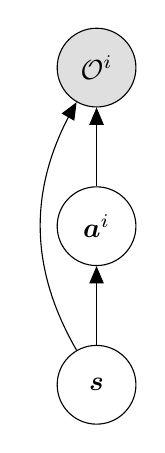
\begin{tikzpicture}[latent/.append style={minimum size=1.0cm}]
        \node[obs] (o) {$\mathcal{O}^i$};
        \node[latent, below=of o] (a) {$\boldsymbol{a}^i$};
        \node[latent, below=of a] (s) {$\boldsymbol{s}$};
    
        \edge {s} {a}
        \edge {a} {o}
        \path[->]  (s)  edge   [bend left=30] node {} (o);
    \end{tikzpicture}
    \end{minipage}%
    \begin{minipage}[t]{0.5\linewidth}
    \captionof{figure}{Graphical model of One-Step Single agent reinforcement learning with visible optimality variable.} 
    \label{fig:one-step-single agent}
    \end{minipage}
\end{figure}
In this case, we can arrive at the same objective as a Lagrange multiplier method. However, for a multi-agent case, strictly speaking, having difference Lagrange multiplier for each of KL-Divergence term (the agent and the opponent) is \emph{impossible} (currently), if we derived the objective from this innocent looking graphical model (see \ref{fig:sad-graphical-balance-q}): 

\begin{figure}[ht]
    \begin{minipage}[t]{0.5\linewidth}
    \centering
    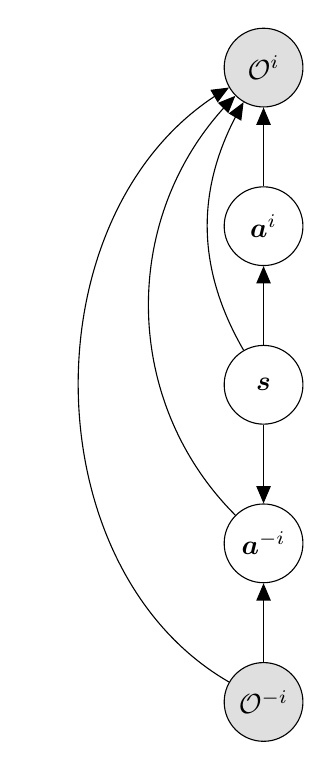
\begin{tikzpicture}[latent/.append style={minimum size=1.0cm}]
        \node[obs] (o) {$\mathcal{O}^i$};
        \node[latent, below=of o] (a) {$\boldsymbol{a}^i$};
        \node[latent, below=of a] (s) {$\boldsymbol{s}$};
        \node[latent, below=of s] (a1) {$\boldsymbol{a}^{-i}$};
        \node[obs, below=of a1] (o1) {$\mathcal{O}^{-i}$};
        
        \edge{o1} {a1}
        \edge {s} {a, a1}
        \edge {a} {o}
        \path[->]  (o1)  edge   [bend left=60] node {} (o);
        \path[->]  (a1)  edge   [bend left=45] node {} (o);
        \path[->]  (s)  edge   [bend left=30] node {} (o);
    \end{tikzpicture}
    \end{minipage}%
    \begin{minipage}[t]{0.5\linewidth}
    \captionof{figure}{Attempt to define Balancing Soft-Q learning via a graphical model. We can see that the optimality of the agent $\mathcal{O}^{i}$ is based on the optionally of other agents $\mathcal{O}^{-i}$. Furthermore, the action of opponent agents is assumed to be optimal.} 
    \label{fig:sad-graphical-balance-q}
    \end{minipage}
\end{figure}
Let's define the joint probability of this graphical model 
\begin{equation}
    \begin{aligned}
        P(\mathcal{O}^i = 1, \boldsymbol{a}^i, \boldsymbol{s}, \boldsymbol{a}^{-i}, \mathcal{O}^{-i} = 1) = &P(\mathcal{O}^i = 1 | \boldsymbol{a}^i, \boldsymbol{s}, \boldsymbol{a}^{-i}, \mathcal{O}^{-i} = 1) \\
        &P_{\text{prior}}(\boldsymbol{a}^i | \boldsymbol{s}) P(\boldsymbol{s}) P_{\text{prior}}(\boldsymbol{a}^{-i} | \boldsymbol{s}, \mathcal{O}^{-i} = 1) P(\mathcal{O}^{-i} = 1)
    \end{aligned}
\end{equation}
Now define the variational distribution. 
\begin{equation}
    \begin{aligned}
        q(\boldsymbol{a}^i, \boldsymbol{s}, \boldsymbol{a}^{-i}, \mathcal{O}^{-i} = 1) = \pi_{\theta} (\boldsymbol{a}^i | \boldsymbol{s}) \rho_{\phi}(\boldsymbol{a}^{-i} | \boldsymbol{s}, \mathcal{O}^{-i} = 1) P(\boldsymbol{s}) P(\mathcal{O}^{-i} = 1)
    \end{aligned}
\end{equation}
Let the optimality of the agent be defined, given that the opponent is optimal, to be  
\begin{equation}
    P(\mathcal{O}^i = 1 | \boldsymbol{a}^i, \boldsymbol{s}, \boldsymbol{a}^{-i}, \mathcal{O}^{-i} = 1) = \exp\Big( \beta R(\boldsymbol{s}, \boldsymbol{a}^i, \boldsymbol{a}^{-i}) \Big)
\end{equation}
Now we can see where the variable $\beta$ is coming from. With this, the ELBO can be found by minimizing KL-Divergence between a variational distribution and joint probability:
\begin{equation*}
    \begin{aligned}
        &\begin{aligned}[t]
            \mathbb{E}_{q(\boldsymbol{a}^i, \boldsymbol{s}, \boldsymbol{a}^{-i}, \mathcal{O}^{-i} = 1)} \bigg[ &\log \pi_{\theta} (\boldsymbol{a}^i | \boldsymbol{s}) + \log \rho_{\phi}(\boldsymbol{a}^{-i} | \boldsymbol{s}, \mathcal{O}^{-i} = 1) + \cancel{\log P(\boldsymbol{s})} + \cancel{\log P(\mathcal{O}^{-i} = 1)}  \\
            &-\log \exp\Big( \beta R(\boldsymbol{s}, \boldsymbol{a}^i, \boldsymbol{a}^{-i}) \Big) - \log P_{\text{prior}}(\boldsymbol{a}^i | \boldsymbol{s}) - \cancel{\log  P(\boldsymbol{s})} \\
            &- \log P_{\text{prior}}(\boldsymbol{a}^{-i} | \boldsymbol{s}, \mathcal{O}^{-i} = 1) -\log \cancel{P(\mathcal{O}^{-i} = 1)} \bigg]
        \end{aligned} \\
        &= \begin{aligned}[t]
            \mathbb{E}_{q(\boldsymbol{a}^i, \boldsymbol{s}, \boldsymbol{a}^{-i}, \mathcal{O}^{-i} = 1)} \bigg[ &- \beta R(\boldsymbol{s}, \boldsymbol{a}^i, \boldsymbol{a}^{-i}) + \log \pi_{\theta} (\boldsymbol{a}^i | \boldsymbol{s}) + \log \rho_{\phi}(\boldsymbol{a}^{-i} | \boldsymbol{s}) \\
            &-\log P_{\text{prior}}(\boldsymbol{a}^i | \boldsymbol{s}) - \log P_{\text{prior}}(\boldsymbol{a}^{-i} | \boldsymbol{s}, \mathcal{O}^{-i} = 1) \bigg]
        \end{aligned}
    \end{aligned}
\end{equation*}
The optimizing objective is 
\begin{equation}
    \mathbb{E}_{q(\boldsymbol{a}^i, \boldsymbol{s}, \boldsymbol{a}^{-i}, \mathcal{O}^{-i} = 1)} \bigg[ R(\boldsymbol{s}, \boldsymbol{a}^i, \boldsymbol{a}^{-i}) + \frac{1}{\beta} \log \frac{\pi_{\theta} (\boldsymbol{a}^i | \boldsymbol{s})}{P_{\text{prior}}(\boldsymbol{a}^i | \boldsymbol{s})}  + \frac{1}{\beta} \log \frac{\rho_{\phi}(\boldsymbol{a}^{-i} | \boldsymbol{s})}{P_{\text{prior}}(\boldsymbol{a}^{-i} | \boldsymbol{s}, \mathcal{O}^{-i} = 1)} \bigg]
\end{equation}
Superficially, the objective looks striking similar to Balancing Soft-Q objective, however, the nature of $\beta$ for each KL-divergence is different.  This leads to an opponent model that resembles the value viewed by the agent since $\beta$ are the same for both agents and opponent model. This leads to the main problem we are trying to solve: \textbf{How to inject the opponent's characteristic into our graphical model without relying on Lagrange multiplier ?}

\begin{tcolorbox}
\textbf{Lesson 2: } Opponent Characteristic can't be represented in centralized graphical model -- a graphical model that unifying every dependency from opponent model to agent's policy -- due to different characteristic of both agent's and opponent's. Balancing Soft-Q works because it contains separate Lagrange multipliers (and 2 stages of optimization)
\end{tcolorbox}

Furthermore, although Lagrange multiplier's method yields very interesting objective, we didn't see any connection between constraint on KL-Divergence to a behaviour of the agent apart from its bounded rationality. This conclusion comes from the same reason KL-Divergence constraints are introduced in the first place -- because we want to limit the rationality of agent alone. 

\begin{tcolorbox}
\textbf{Lesson 3: }Lagrange multiplier's method doesn't make a lot of senses (explanation needed) + not extensible, therefore we need a graphical model to explain this.
\end{tcolorbox}
\emph{\textbf{Note}: Balancing Soft-Q still got other problems, which we explored later.}  

\subsection{Deriving Optimal Policy for Balancing Soft-Q}
Let's see how to derive the optimal policy from the objective. This will be a common pattern when we derive other algorithms. Furthermore, this is based on \cite{levine2018reinforcement} message passing, however, considering only the base case. We would like to find the optimal opponent by maximising the following objective with respect to $\rho_{\phi}$ (We also define a normalizing term/message to be $N(\boldsymbol{s}, \boldsymbol{a}^i)$. The real definition will be clear afterwards)

\begin{equation*}
    \begin{aligned}
        \mathbb{E}_{q(\boldsymbol{s}, \boldsymbol{a}^i)}&\bigg[ \mathbb{E}_{q(\boldsymbol{a}^{-i} | \boldsymbol{s})} \bigg[ R(\boldsymbol{s}, \boldsymbol{a}^i, \boldsymbol{a}^{-i}) - \frac{1}{\beta_{-i}}\log \frac{\rho_{\phi}(\boldsymbol{a}^i | \boldsymbol{s})}{P_{\text{prior}}(\boldsymbol{a}^{-i} | \boldsymbol{s})}  \bigg] - \frac{1}{\beta_{i}}\log \frac{\pi_{\theta}(\boldsymbol{a}^i | \boldsymbol{s})}{P_{\text{prior}}(\boldsymbol{a}^i | \boldsymbol{s})} \bigg] \\
        &= \begin{aligned}[t]
            \mathbb{E}_{q(\boldsymbol{s}, \boldsymbol{a}^i)} \bigg[ \mathbb{E}_{q(\boldsymbol{a}^{-i} | \boldsymbol{s})} \bigg[ R&(\boldsymbol{s}, \boldsymbol{a}^i, \boldsymbol{a}^{-i}) - \frac{1}{\beta_{-i}}\log \rho_{\phi}(\boldsymbol{a}^i | \boldsymbol{s})  \\
            &+\frac{1}{\beta_{-i}} \log P_{\text{prior}}(\boldsymbol{a}^{-i} | \boldsymbol{s}) - N(\boldsymbol{s}, \boldsymbol{a}^{i}) + N(\boldsymbol{s}, \boldsymbol{a}^{i}) \bigg] \\
            &+\frac{1}{\beta_{i}}\log \frac{\pi_{\theta}(\boldsymbol{a}^i | \boldsymbol{s})}{P_{\text{prior}}(\boldsymbol{a}^i | \boldsymbol{s})} \bigg]
        \end{aligned} \\
        &= \begin{aligned}[t]
            \mathbb{E}_{q(\boldsymbol{s}, \boldsymbol{a}^i, \boldsymbol{a}^{-i})}[N(\boldsymbol{s}, \boldsymbol{a}^i)] - \mathbb{E}_{q(\boldsymbol{s}, \boldsymbol{a}^i)} \bigg[ \mathbb{E}_{q(\boldsymbol{a}^{-i} | \boldsymbol{s})} \bigg[ -R&(\boldsymbol{s}, \boldsymbol{a}^i, \boldsymbol{a}^{-i}) + \frac{1}{\beta_{-i}}\log \rho_{\phi}(\boldsymbol{a}^i | \boldsymbol{s})  \\
            &-\frac{1}{\beta_{-i}} \log P_{\text{prior}}(\boldsymbol{a}^{-i} | \boldsymbol{s})+ N(\boldsymbol{s}, \boldsymbol{a}^{i}) \bigg] \\
            &+\frac{1}{\beta_{i}}\log \frac{\pi_{\theta}(\boldsymbol{a}^i | \boldsymbol{s})}{P_{\text{prior}}(\boldsymbol{a}^i | \boldsymbol{s})}\bigg]
        \end{aligned} \\
        &= \begin{aligned}[t]
            \mathbb{E}_{q(\boldsymbol{s}, \boldsymbol{a}^i, \boldsymbol{a}^{-i})}[N(\boldsymbol{s}, \boldsymbol{a}^i)] - \mathbb{E}_{q(\boldsymbol{s}, \boldsymbol{a}^i)} \bigg[ \mathbb{E}_{q(\boldsymbol{a}^{-i} | \boldsymbol{s})} \bigg[ -\beta_{-i} R&(\boldsymbol{s}, \boldsymbol{a}^i, \boldsymbol{a}^{-i}) + \log \rho_{\phi}(\boldsymbol{a}^i | \boldsymbol{s})  \\
            &-\log P_{\text{prior}}(\boldsymbol{a}^{-i} | \boldsymbol{s})+ N(\boldsymbol{s}, \boldsymbol{a}^{i}) \bigg] \\
            &+\frac{\beta_{-i}}{\beta_{i}}\log \frac{\pi_{\theta}(\boldsymbol{a}^i | \boldsymbol{s})}{P_{\text{prior}}(\boldsymbol{a}^i | \boldsymbol{s})}\bigg]
        \end{aligned}  \\
        &= \begin{aligned}[t]
            \mathbb{E}_{q(\boldsymbol{s}, \boldsymbol{a}^i, \boldsymbol{a}^{-i})}[N(\boldsymbol{s}, \boldsymbol{a}^i)] - \mathbb{E}_{q(\boldsymbol{s}, \boldsymbol{a}^i)} \bigg[ \mathbb{E}_{q(\boldsymbol{a}^{-i} | \boldsymbol{s})} \bigg[ &\log \rho_{\phi}(\boldsymbol{a}^i | \boldsymbol{s}) \\
            &-\bigg[ \beta_{-i} R(\boldsymbol{s}, \boldsymbol{a}^i, \boldsymbol{a}^{-i})   +\log P_{\text{prior}}(\boldsymbol{a}^{-i} | \boldsymbol{s}) - 
            N(\boldsymbol{s}, \boldsymbol{a}^{i}) \bigg] \bigg] \\
            &+\frac{\beta_{-i}}{\beta_{i}}\log \frac{\pi_{\theta}(\boldsymbol{a}^i | \boldsymbol{s})}{P_{\text{prior}}(\boldsymbol{a}^i | \boldsymbol{s})}\bigg]
        \end{aligned} \\
        &= \begin{aligned}[t]
            \mathbb{E}_{q(\boldsymbol{s}, \boldsymbol{a}^i, \boldsymbol{a}^{-i})}[ N(\boldsymbol{s}, \boldsymbol{a}^i)] - \mathbb{E}_{q(\boldsymbol{s}, \boldsymbol{a}^i)} \Bigg[ &D_{KL}\Bigg[ \rho_{\phi}(\boldsymbol{a}^i | \boldsymbol{s}) \Bigg|\Bigg| \frac{\exp(\beta_{-i} R(\boldsymbol{s}, \boldsymbol{a}^i, \boldsymbol{a}^{-i}))P_{\text{prior}}(\boldsymbol{a}^{-i} | \boldsymbol{s})}{\exp N(\boldsymbol{s}, \boldsymbol{a}^{i})} \Bigg] \Bigg] \\  &+\frac{\beta_{-i}}{\beta_{i}}\log \frac{\pi_{\theta}(\boldsymbol{a}^i | \boldsymbol{s})}{P_{\text{prior}}(\boldsymbol{a}^i | \boldsymbol{s})}\bigg]
        \end{aligned} 
    \end{aligned}
\end{equation*}
\textbf{Note: } We absolve the constant $\beta_{-i}$ inside the normalizing factor. The optimal opponent is then equal to (There is a problem with $\boldsymbol{a}^i$. However, we care about using its policy to find the final value.)
\begin{equation}
    \rho_{\phi}(\boldsymbol{a}^{-i} | \boldsymbol{s}) = \frac{\exp(\beta_{-i} R(\boldsymbol{s}, \boldsymbol{a}^i, \boldsymbol{a}^{-i}))P_{\text{prior}}(\boldsymbol{a}^{-i} | \boldsymbol{s})}{\exp N(\boldsymbol{s}, \boldsymbol{a}^{i})}
\end{equation}
This also leads to a normalizing factor of 
\begin{equation}
    N(\boldsymbol{s}, \boldsymbol{a}^{i}) = \frac{1}{\beta_{-i} }\log \int_{\mathcal{A}^{-i}} \exp(R(\boldsymbol{s}, \boldsymbol{a}^i, \boldsymbol{a}^{-i}))P_{\text{prior}}(\boldsymbol{a}^{-i} | \boldsymbol{s})
\end{equation}
We can interpret this as the game's Q-value function based on prior knowledge of opponent \cite{grau2018balancing} in the view of agent's. After getting the optimal opponent that is solely based on $R(\boldsymbol{s}, \boldsymbol{a}, \boldsymbol{a}^{-i})$, now we can find the agent optimal policy by substitute this optimal opponent back, and optimize the agent's policy instead.

\begin{equation*}
    \begin{aligned}
        &\mathbb{E}_{q(\boldsymbol{s}, \boldsymbol{a}^i, \boldsymbol{a}^{-i})}\bigg[ R(\boldsymbol{s}, \boldsymbol{a}^i, \boldsymbol{a}^{-i})  - \frac{1}{\beta_{i}}\log \frac{\pi_{\theta}(\boldsymbol{a}^i | \boldsymbol{s})}{P_{\text{prior}}(\boldsymbol{a}^i | \boldsymbol{s})}  - \frac{1}{\beta_{-i}}\log \frac{\exp(\beta_{-i} R(\boldsymbol{s}, \boldsymbol{a}^i, \boldsymbol{a}^{-i}))\cancel{P_{\text{prior}}(\boldsymbol{a}^{-i} | \boldsymbol{s})}}{\exp  N(\boldsymbol{s}, \boldsymbol{a}^{i}) \cancel{P_{\text{prior}}(\boldsymbol{a}^{-i} | \boldsymbol{s})} } \bigg] \\
        &= \mathbb{E}_{q(\boldsymbol{s}, \boldsymbol{a}^i, \boldsymbol{a}^{-i})}\bigg[ \cancel{R(\boldsymbol{s}, \boldsymbol{a}^i, \boldsymbol{a}^{-i})}  - \frac{1}{\beta_{i}}\log \frac{\pi_{\theta}(\boldsymbol{a}^i | \boldsymbol{s})}{P_{\text{prior}}(\boldsymbol{a}^i | \boldsymbol{s})}  - \cancel{R(\boldsymbol{s}, \boldsymbol{a}^i, \boldsymbol{a}^{-i}))} + \underbrace{ \frac{1}{\beta_{-i}}\log \exp N(\boldsymbol{s}, \boldsymbol{a}^{i})}_{R(\boldsymbol{s}, \boldsymbol{a}^i)} \bigg]\\
        &= \mathbb{E}_{q(\boldsymbol{s}, \boldsymbol{a}^i, \boldsymbol{a}^{-i})}\bigg[ \beta_i R(\boldsymbol{s}, \boldsymbol{a}^i) - \log \pi_{\theta}(\boldsymbol{a}^i | \boldsymbol{s}) +  P_{\text{prior}}(\boldsymbol{a}^i | \boldsymbol{s}) + N(\boldsymbol{s}) - N(\boldsymbol{s}) \bigg] \\
        &= \mathbb{E}_{q(\boldsymbol{s}, \boldsymbol{a}^i, \boldsymbol{a}^{-i})}[N(\boldsymbol{s})] - 
        \mathbb{E}_{q(\boldsymbol{s}, \boldsymbol{a}^i, \boldsymbol{a}^{-i})}\bigg[ -\beta_i R(\boldsymbol{s}, \boldsymbol{a}^i) + \log \pi_{\theta}(\boldsymbol{a}^i | \boldsymbol{s}) -  P_{\text{prior}}(\boldsymbol{a}^i | \boldsymbol{s}) + N(\boldsymbol{s}) \bigg] \\
        &= \mathbb{E}_{q(\boldsymbol{s}, \boldsymbol{a}^i, \boldsymbol{a}^{-i})}[N(\boldsymbol{s})] - 
        \mathbb{E}_{q(\boldsymbol{s}, \boldsymbol{a}^i, \boldsymbol{a}^{-i})}\bigg[\log \pi_{\theta}(\boldsymbol{a}^i | \boldsymbol{s}) - \bigg[\beta_i R(\boldsymbol{s}, \boldsymbol{a}^i) +P_{\text{prior}}(\boldsymbol{a}^i | \boldsymbol{s}) -  N(\boldsymbol{s}) \bigg] \bigg] \\
        &= \mathbb{E}_{q(\boldsymbol{s}, \boldsymbol{a}^i \boldsymbol{a}^{-i})}[N(\boldsymbol{s})] - 
        \mathbb{E}_{q(\boldsymbol{s},  \boldsymbol{a}^{-i})}\bigg[D_{KL}\bigg[ \log \pi_{\theta}(\boldsymbol{a}^i | \boldsymbol{s}) \bigg|\bigg| \frac{\exp\left( \beta_i R(\boldsymbol{s}, \boldsymbol{a}^i)\right) P_{\text{prior}}(\boldsymbol{a}^i | \boldsymbol{s})}{N(\boldsymbol{s})}  \bigg]\bigg]
    \end{aligned} 
\end{equation*}
In order to max the objective we have to set $\pi_{\theta}$ to be equal to 

\begin{equation*}
    \pi_{\theta}(\boldsymbol{a}^i | \boldsymbol{s}) = \frac{\exp\left( \beta_i R(\boldsymbol{s}, \boldsymbol{a}^i)\right) P_{\text{prior}}(\boldsymbol{a}^i | \boldsymbol{s})}{N(\boldsymbol{s})}
\end{equation*}
This corresponds directly to \cite{grau2018balancing} optimal policy. However, if we can see, the term $R(\boldsymbol{s}, \boldsymbol{a}^i, \boldsymbol{a}^{-i})$ got cancelled due to the Lagrange multiplier on $\log \frac{\rho_{\phi}(\boldsymbol{a}^i | \boldsymbol{s})}{P_{\text{prior}}(\boldsymbol{a}^{-i} | \boldsymbol{s})}$. With this observation and our derivation of Balancing Soft-Q, we can conclude that: 

\begin{tcolorbox}
\textbf{Lesson 4: }\label{lesson:4} We need to have an \textbf{independent inference method for calculating opponent's model}. \cite{grau2018balancing} works can be seen as non-decentralized version of ROMMEO (since we directly use \textit{opponent's optimal policy against agent's prior or simply ignore it} the agent's policy should be $\pi(\boldsymbol{a}^i | \boldsymbol{s}, \boldsymbol{a}^{-i})$)
\end{tcolorbox}

\begin{tcolorbox}
\textbf{Lesson 5: } There are 2 steps we have to make: first finding the extreme case of the value function, then we can find a policy.  
\end{tcolorbox}

\section{Unified View}

\noindent
The reasoning is the following, which is repeatable.
\begin{enumerate}
    \item We assume we know the optimal opponent model $\rho_{\phi}(\boldsymbol{a}^{-i}_t | \boldsymbol{s}_t)$, at first iteration it can be just a \textbf{prior} of the opponent of the agent.  
    \item After we found the optimal agent model, we can now find the agent  $\pi_{\theta}(\boldsymbol{a}^i_t | \boldsymbol{a}^{-i}_t, \boldsymbol{s}_t)$. This is analogous to the $\text{ext}_{\pi_{\theta}}$ operation in \cite{grau2018balancing}
    \item We can use the result from the optimal agent model $\pi_{\theta}(\boldsymbol{a}^i_t | \boldsymbol{a}^{-i}_t, \boldsymbol{s}_t)$ to find **better** optimal opponent model. (\textbf{Might need a proof of improvement}). This is analogous to $\arg\max_{\rho}$ operation
    \item We are not sure its connection to the fictitious play in \cite{1591992}. 
\end{enumerate}

\subsection{Deriving Agent's Policy}
Starting with finding the agent's policy: 

\begin{figure}[ht]
    \begin{minipage}[t]{0.5\linewidth}
    \centering
    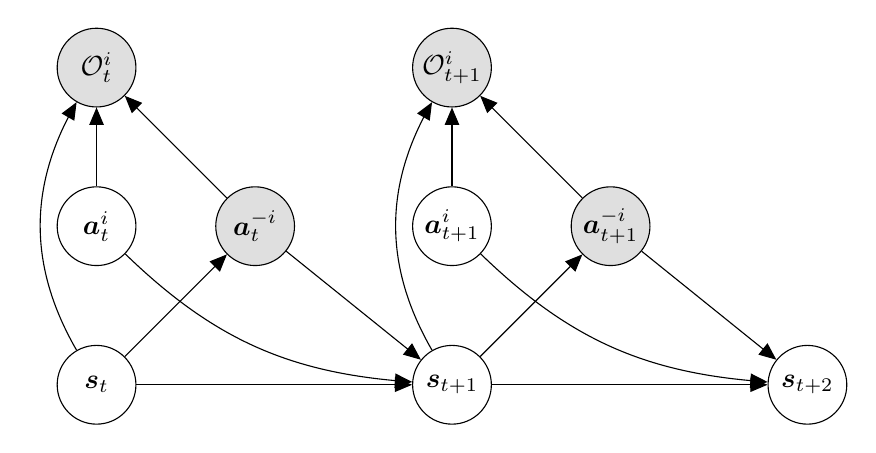
\begin{tikzpicture}[latent/.append style={minimum size=1.0cm}]
        \node[obs] (ot) {$\mathcal{O}^{i}_t$};
        \node[latent, below=of ot] (at) {$\boldsymbol{a}^{i}_t$};
        \node[latent, below=of at] (st) {$\boldsymbol{s}_t$};
        \node[obs, right=of at] (a1t) {$\boldsymbol{a}^{-i}_t$};
        
        \node[latent, right=3.5cm of st] (st1) {$\boldsymbol{s}_{t+1}$};
        \node[latent, above=of st1] (at1) {$\boldsymbol{a}^{i}_{t+1}$};
        
        \node[obs, above=of at1] (ot1) {$\mathcal{O}^{i}_{t+1}$};
        \node[obs, right=of at1] (a1t1) {$\boldsymbol{a}^{-i}_{t+1}$};
        \node[latent, right=3.5cm of st1] (st2) {$\boldsymbol{s}_{t+2}$};        
        % above right=1.3cm of a
        \edge {at, a1t} {ot}
        \edge {st, a1t} {st1}
        \edge {st} {a1t}
        
        \edge{at1, a1t1} {ot1}
        \edge{st1} {a1t1}
        
        \edge {st1, a1t1} {st2}
        
        \path[->]  (st)  edge   [bend left=30] node {} (ot);
        \path[->]  (st1)  edge   [bend left=30] node {} (ot1);
        \path[->]  (at)  edge   [bend right=20] node {} (st1);
        
        \path[->]  (at1)  edge   [bend right=20] node {} (st2);
    \end{tikzpicture}
    \end{minipage}%
    \begin{minipage}[t]{0.5\linewidth}
    \captionof{figure}{Graphical model. We want to approximate. We assume that we knows what the opponent should be. In this case, we know the opponent model} 
    \end{minipage}
\end{figure}
\noindent
We can see that the joint probability is equal to 
\begin{equation}
    \begin{aligned}
        P(\mathcal{O}^i_{1:T} = 1, \boldsymbol{s}_{1:T}, \boldsymbol{a}^i_{1:T}, \boldsymbol{a}^{-i}_{1:T}) = P(\boldsymbol{s}_1) \prod^T_{t=1} &P(\mathcal{O}^i_{t} = 1 | \boldsymbol{s}_{t}, \boldsymbol{a}^i_{t}, \boldsymbol{a}^{-i}_{t}) P_{\text{prior}}(\boldsymbol{a}^i_t) \\
        &P(\boldsymbol{s}_{t+1} | \boldsymbol{s}_{t}, \boldsymbol{a}^i_{t}, \boldsymbol{a}^{-i}_{t})  \rho_{\phi}(\boldsymbol{a}^{-i}_t | \boldsymbol{s}_t)
    \end{aligned}
\end{equation}
We will define the optimality of the agent to be equal to
\begin{equation}
    P(\mathcal{O}_{t} = 1 | \boldsymbol{s}_{t}, \boldsymbol{a}^i_{t}, \boldsymbol{a}^{-i}_{t}) \propto \exp\left( \beta_i R_G(\boldsymbol{s}_{t}, \boldsymbol{a}^i_{t}, \boldsymbol{a}^{-i}_{t}) \right)
\end{equation}
It can be interpreted as a best response toward known opponent (aren't that what we want ? Now the performance of our agent is based on the quality of opponent model). Interestingly, we should consider the case where the opponent is totally difference from out model. Now we shall define the graphical model that we will used to approximate this using variational inference.
\begin{figure}[H]
    \begin{minipage}[t]{0.5\linewidth}
    \centering
    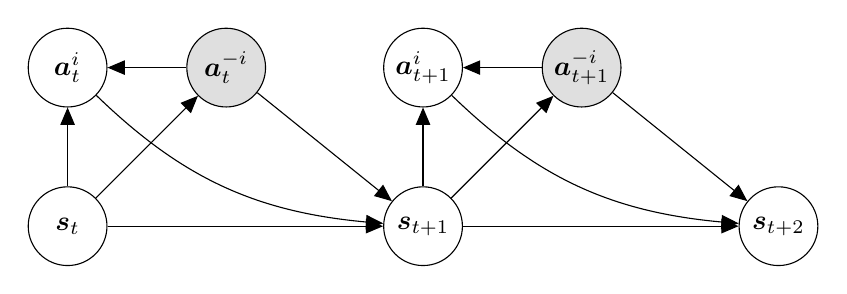
\begin{tikzpicture}[latent/.append style={minimum size=1.0cm}]
        \node[latent] (st) {$\boldsymbol{s}_t$};
        \node[latent, above=of st] (at) {$\boldsymbol{a}^{i}_t$};
        \node[obs, right=of at] (a1t) {$\boldsymbol{a}^{-i}_t$};
        
        \node[latent, right=3.5cm of st] (st1) {$\boldsymbol{s}_{t+1}$};
        \node[latent, above=of st1] (at1) {$\boldsymbol{a}^{i}_{t+1}$};
        
        \node[obs, right=of at1] (a1t1) {$\boldsymbol{a}^{-i}_{t+1}$};
        \node[latent, right=3.5cm of st1] (st2) {$\boldsymbol{s}_{t+2}$};        
        % above right=1.3cm of a
        \edge {st, a1t} {st1}
        \edge {st} {a1t, at}
        \edge {a1t} {at}
        \edge {a1t1} {at1}
        
        \edge{st1} {a1t1, at1}
        \edge {st1, a1t1} {st2}
        
        \path[->]  (at)  edge   [bend right=20] node {} (st1);
        \path[->]  (at1)  edge   [bend right=20] node {} (st2);
    \end{tikzpicture}
    \end{minipage}%
    \begin{minipage}[t]{0.5\linewidth}
    \captionof{figure}{\label{fig:agent-optimal}Graphical model that we will fit $\pi_{\theta}$ to get the optimal agent policy.} 
    \end{minipage}
\end{figure}

\noindent
The joint probability that we will use to approximate 
\begin{equation}
    \begin{aligned}
        q(\boldsymbol{s}_{1:T}, \boldsymbol{a}^i_{1:T}, \boldsymbol{a}^{-i}_{1:T}) = P(\boldsymbol{s}_1) \prod^T_{t=1}
        P(\boldsymbol{s}_{t+1} | \boldsymbol{s}_{t}, \boldsymbol{a}^i_{t}, \boldsymbol{a}^{-i}_{t}) \pi_{\theta}(\boldsymbol{a}^i_t | \boldsymbol{s}_t, \boldsymbol{a}^{-i}_t) \rho_{\phi}(\boldsymbol{a}^{-i}_t | \boldsymbol{s}_t)
    \end{aligned}
\end{equation}
(\emph{Note: } $\rho_{\phi}(\boldsymbol{a}^{-i}_t | \boldsymbol{s}_t)$ represents our assumed opponent model.) Now let's do variational inference by finding ELBO, and then we optimize the ELBO and find the closed form.
\begin{equation}
    \label{equation:4}
    \begin{aligned}
        \log P(\mathcal{O}^i_{1:T} = 1) &= \log \int P(\mathcal{O}^i_{1:T} = 1, \boldsymbol{s}_{1:T}, \boldsymbol{a}^i_{1:T}, \boldsymbol{a}^{-i}_{1:T}) \ d\boldsymbol{s}_{1:T} \ d\boldsymbol{a}^i_{1:T} \ d\boldsymbol{a}^{-i}_{1:T} \\ 
        &= \log \int P(\mathcal{O}^i_{1:T} = 1, \boldsymbol{s}_{1:T}, \boldsymbol{a}^i_{1:T}, \boldsymbol{a}^{-i}_{1:T}) \frac{q(\boldsymbol{s}_{1:T}, \boldsymbol{a}^i_{1:T}, \boldsymbol{a}^{-i}_{1:T})}{q(\boldsymbol{s}_{1:T}, \boldsymbol{a}^i_{1:T}, \boldsymbol{a}^{-i}_{1:T})} \ d\boldsymbol{s}_{1:T} \ d\boldsymbol{a}^i_{1:T} \ d\boldsymbol{a}^{-i}_{1:T} \\
        &\ge \mathbb{E}_{q(\boldsymbol{s}_{1:T}, \boldsymbol{a}^i_{1:T}, \boldsymbol{a}^{-i}_{1:T})}\Bigg[ \log \frac{P(\mathcal{O}^i_{1:T} = 1, \boldsymbol{s}_{1:T}, \boldsymbol{a}^i_{1:T}, \boldsymbol{a}^{-i}_{1:T})}{q(\boldsymbol{s}_{1:T}, \boldsymbol{a}^i_{1:T}, \boldsymbol{a}^{-i}_{1:T})} \Bigg] \\
        &= \mathbb{E}_{q(\boldsymbol{s}_{1:T}, \boldsymbol{a}^i_{1:T}, \boldsymbol{a}^{-i}_{1:T})}\Bigg[\sum^{T}_{t=1} \ \beta_i R_G(\boldsymbol{s}_{t}, \boldsymbol{a}^i_{t}, \boldsymbol{a}^{-i}_{t}) - \log \frac{\pi_{\theta}(\boldsymbol{a}^i_t | \boldsymbol{s}_t, \boldsymbol{a}^{-i}_t)}{P_{\text{prior}}(\boldsymbol{a}^i_t)}\Bigg]
    \end{aligned}
\end{equation}
We refer to section \ref{ELBO:agent} for more detailed proof of ELBO.
Let's derive the closed form solution by following \cite{levine2018reinforcement}. Starting with the base case (at termination). We want to maximize the following objective: 
\begin{equation}
    \mathbb{E}_{q(\boldsymbol{s}_{T}, \boldsymbol{a}^i_{T}, \boldsymbol{a}^{-i}_{T})} \Bigg[\beta_i R_G(\boldsymbol{s}_{T}, \boldsymbol{a}^i_{T}, \boldsymbol{a}^{-i}_{T}) - \log \frac{\pi_{\theta}(\boldsymbol{a}^i_T | \boldsymbol{s}_T, \boldsymbol{a}^{-i}_T)}{P_{\text{prior}}(\boldsymbol{a}^i_T)}\Bigg]
\end{equation}
Let's introduce message $Q^{i}(\boldsymbol{s}_T, \boldsymbol{a}^{-i}_T)$. It will be clear why we introduce such a value and what value it is, later. 
\begin{equation}
    \mathbb{E}_{q(\boldsymbol{s}_{T}, \boldsymbol{a}^i_{T}, \boldsymbol{a}^{-i}_{T})} \Bigg[\beta_i R_G(\boldsymbol{s}_{T}, \boldsymbol{a}^i_{T}, \boldsymbol{a}^{-i}_{T}) - \log \frac{\pi_{\theta}(\boldsymbol{a}^i_T | \boldsymbol{s}_T, \boldsymbol{a}^{-i}_T)}{P_{\text{prior}}(\boldsymbol{a}^i_T)} - Q^{i}(\boldsymbol{s}_T, \boldsymbol{a}^{-i}_T) + Q^{i}(\boldsymbol{s}_T, \boldsymbol{a}^{-i}_T)\Bigg]
\end{equation}
With some algebraic manipulations, we arrived at the following form 
\begin{equation}
    \mathbb{E}_{q(\boldsymbol{s}_{T}, \boldsymbol{a}^{-i}_{T})} \Bigg[ -D_{KL} \Bigg( \pi_{\theta}(\boldsymbol{a}^i_T | \boldsymbol{s}_T, \boldsymbol{a}_T^{-i}) \Bigg|\Bigg| \frac{\exp(\beta_i R_G(\boldsymbol{s}_{T}, \boldsymbol{a}^i_{T}, \boldsymbol{a}^{-i}_{T})) P_{\text{prior}}(\boldsymbol{a}^i_T)}{\exp(N(\boldsymbol{s}_T, \boldsymbol{a}^{-i}_T))} \Bigg) + Q^{i}(\boldsymbol{s}_T, \boldsymbol{a}^{-i}_T) \Bigg]
\end{equation}
If we want to maximize the following objective, we have to set KL-Divergence to be zero meaning that we set $\pi_{\theta}$ to be equal to 
\begin{equation}
    \pi_{\theta}(\boldsymbol{a}^i_T | \boldsymbol{s}_T, \boldsymbol{a}_T^{-i}) = \frac{\exp(\beta_i R_G(\boldsymbol{s}_{T}, \boldsymbol{a}^i_{T}, \boldsymbol{a}^{-i}_{T})) P_{\text{prior}}(\boldsymbol{a}^i_T)}{\exp(Q^{i}(\boldsymbol{s}_T, \boldsymbol{a}^{-i}_T))}
\end{equation}
Where we set the normalizing term to be equal to 
\begin{equation}
    Q^{i}(\boldsymbol{s}_T, \boldsymbol{a}^{-i}_T) = \log \int \exp(\beta_i R_G(\boldsymbol{s}_{T}, \boldsymbol{a}^i_{T}, \boldsymbol{a}^{-i}_{T})) P_{\text{prior}}(\boldsymbol{a}^i_T) \ d \boldsymbol{a}^i_T
\end{equation}
After maximizing, we are left with $N(\boldsymbol{s}_T, \boldsymbol{a}^{-i}_T)$, in which we carry this term to the step before. Now, for arbitrary time-step $t$, we can now derive the closed form solution of $\pi_{\theta}$. Getting the objective (introducing $Q^{i}(\boldsymbol{s}_t, \boldsymbol{a}^{-i}_t)$ is hidden but the steps are the same):
\begin{equation}
    \begin{aligned}
        \mathbb{E}_{q(\boldsymbol{s}_{t}, \boldsymbol{a}^i_{t}, \boldsymbol{a}^{-i}_{t})} \Bigg[\underbrace{\beta_i R_G(\boldsymbol{s}_{t}, \boldsymbol{a}^i_{t}, \boldsymbol{a}^{-i}_{t}) + \gamma\mathbb{E}_{P(\boldsymbol{s}_{t+1}, \boldsymbol{a}^{-i}_{t+1} | \boldsymbol{a}^{i}_{t})}\Big[ Q^{i}(\boldsymbol{s}_{t+1}, \boldsymbol{a}^{-i}_{t+1}) \Big]}_{Q^i(\boldsymbol{s}_t, \boldsymbol{a}^i_t, \boldsymbol{a}^{-i}_t)} - \log \frac{\pi_{\theta}(\boldsymbol{a}^i_t | \boldsymbol{s}_t, \boldsymbol{a}^{-i}_t)}{P_{\text{prior}}(\boldsymbol{a}^i_t)} \Bigg]
    \end{aligned}
\end{equation}
Noted that our choice for opponent's policy is embedded, within 
\begin{equation}
    P(\boldsymbol{s}_{t+1}, \boldsymbol{a}^{-i}_{t+1} | \boldsymbol{a}^{i}_{t}) = P(\boldsymbol{s}_{t+1} | \boldsymbol{s}_t, \boldsymbol{a}^i_t, \boldsymbol{a}^{-i}_t) \rho_{\phi}(\boldsymbol{a}^{-i}_{t+1} | \boldsymbol{s}_{t+1})
\end{equation}
Following the same procedure, as above, we can set $\pi_{\theta}$ to be equal to 
\begin{equation}
    \pi_{\theta}(\boldsymbol{a}^i_T | \boldsymbol{s}_T, \boldsymbol{a}_T^{-i}) = \frac{\exp(Q(\boldsymbol{s}_t, \boldsymbol{a}^i_t, \boldsymbol{a}^{-i}_t)) P_{\text{prior}}(\boldsymbol{a}^i_T)}{\exp(Q^{i}(\boldsymbol{s}_t, \boldsymbol{a}^{-i}_t))}
\end{equation}
Where, 
\begin{equation}
    \begin{aligned}
        &Q^i(\boldsymbol{s}_t, \boldsymbol{a}^i_t, \boldsymbol{a}^{-i}_t) = \beta_i R_G(\boldsymbol{s}_{t}, \boldsymbol{a}^i_{t}, \boldsymbol{a}^{-i}_{t}) + \gamma \mathbb{E}_{P(\boldsymbol{s}_{t+1}, \boldsymbol{a}^{-i}_{t+1})}\Big[ Q^{i} (\boldsymbol{s}_{t+1}, \boldsymbol{a}^{-i}_{t+1}) \Big] \\
        & Q^{i}(\boldsymbol{s}_t, \boldsymbol{a}^{-i}_t) = \log \int \exp(Q(\boldsymbol{s}_t, \boldsymbol{a}^i_t, \boldsymbol{a}^{-i}_t)) P_{\text{prior}}(\boldsymbol{a}^i_T) \ d \boldsymbol{a}^i_t
    \end{aligned}
\end{equation}

\subsection{Deriving Opponent's Policy}
After we can get a hold of the agent's policy, we can now find the opponent model. Let's show the graphical model that we want to approximate. 

\begin{figure}[ht]
    \begin{minipage}[t]{0.5\linewidth}
    \centering
    \begin{tikzpicture}[latent/.append style={minimum size=1.0cm}]
        \node[obs] (o1t) {$\mathcal{O}^{-i}_t$};
        \node[latent, below=of o1t] (a1t) {$\boldsymbol{a}^{-i}_t$};
        \node[latent, right=of a1t] (at) {$\boldsymbol{a}^{i}_t$};
        \node[latent, below=of a1t] (st) {$\boldsymbol{s}_t$};
        
        \node[latent, right=3.5cm of st] (st1) {$\boldsymbol{s}_{t+1}$};
        
        \node[latent, above=of st1] (a1t1) {$\boldsymbol{a}^{-i}_{t+1}$};
        \node[obs, above=of a1t1] (o1t1) {$\mathcal{O}^{-i}_{t+1}$};
        \node[latent, right=of a1t1] (at1) {$\boldsymbol{a}^{i}_{t+1}$};
        \node[latent, right=3.5cm of st1] (st2) {$\boldsymbol{s}_{t+2}$}; 
        
        % above right=1.3cm of a
        \edge {a1t} {o1t}
        \edge {a1t} {at}
        \edge {a1t1} {at1}
        \edge {st, at} {st1}
        \edge {st} {at}
        \edge {st1} {at1}
        \edge {st1, at1} {st2}
        \edge {a1t1} {o1t1}
        
        
        \path[->]  (st)  edge   [bend left=30] node {} (o1t);
        \path[->]  (st1)  edge   [bend left=30] node {} (ot1);
        \path[->]  (a1t)  edge   [bend right=20] node {} (st1);
        \path[->]  (a1t1)  edge   [bend right=20] node {} (st2);
    \end{tikzpicture}
    \end{minipage}%
    \begin{minipage}[t]{0.5\linewidth}
    \captionof{figure}{Graphical model. Now we know that agent's policy, we would like to find a better opponent model.} 
    \end{minipage}
\end{figure}

\noindent
The joint probability is defined to be 
\begin{equation}
    \begin{aligned}
        P(\mathcal{O}^{-i}_{1:T} = 1, \boldsymbol{s}_{1:T}, \boldsymbol{a}^i_{1:T}, \boldsymbol{a}^{-i}_{1:T}) = P(\boldsymbol{s}_1) \prod^T_{t=1} &P(\mathcal{O}^{-i}_{t} = 1 | \boldsymbol{s}_{t}, \boldsymbol{a}^{-i}_{t}) P_{\text{prior}}(\boldsymbol{a}^{-i}_t) \\
        &P(\boldsymbol{s}_{t+1} | \boldsymbol{s}_{t}, \boldsymbol{a}^i_{t}, \boldsymbol{a}^{-i}_{t}) \pi_{\theta}(\boldsymbol{a}^{i}_t | \boldsymbol{s}_t, \boldsymbol{a}^{-i}_t)
    \end{aligned}
\end{equation}
Since, we already know what our agent's policy is. The optimally of the opponent model shall be equal to expectation of reward received by opponent, given agent's policy. 
\begin{equation}
    \begin{aligned}
        P(\mathcal{O}^{-i}_{t} = 1 | \boldsymbol{s}_{t}, \boldsymbol{a}^{-i}_{t}) = \exp\left(R^{-i}(\boldsymbol{s}_t, \boldsymbol{a}^{-i}_t)\right)
    \end{aligned}
\end{equation}
The definition of $R^{-i}(\boldsymbol{s}_t, \boldsymbol{a}_t^{-i})$ stills be ambiguous, however, the first definition posts more promising approach that is because we define the joint probability $P(\mathcal{O}^{-i}_{1:T} = 1, \boldsymbol{s}_{1:T}, \boldsymbol{a}^i_{1:T}, \boldsymbol{a}^{-i}_{1:T})$ to be related to $\pi_{\theta}(\boldsymbol{a}^{i}_t | \boldsymbol{s}_t, \boldsymbol{a}^{-i}_t)$. Unless, we include the prior of agent's policy $P_{\text{prior}}$ within the graphical model. (Noted that in \cite{grau2018balancing} they has used the second equation, since they assume that the opponent doesn't know the true policy, hence using the prior.)
\begin{equation}
    \begin{aligned}
        \int \beta_{-i}R_G(\boldsymbol{s}_t, \boldsymbol{a}_t, \boldsymbol{a}^{-i}_t) \pi_{\theta}(\boldsymbol{a}^i_t | \boldsymbol{a}^{-i}_t, \boldsymbol{s}_t) \ d\boldsymbol{a}^i_t \quad \text{ or } \quad
        \int \beta_{-i}R_G(\boldsymbol{s}_t, \boldsymbol{a}_t, \boldsymbol{a}^{-i}_t) P_{\text{prior}}(\boldsymbol{a}^i_t) \ d\boldsymbol{a}^i_t 
    \end{aligned}
\end{equation}
Now, the graphical model that we want to fit is almost the same in agent's case. However, now we know the agent, but not opponent model (noted that we might absolve the agent's policy within the enviornment dynamic)
\begin{figure}[H]
    \begin{minipage}[t]{0.5\linewidth}
    \centering
    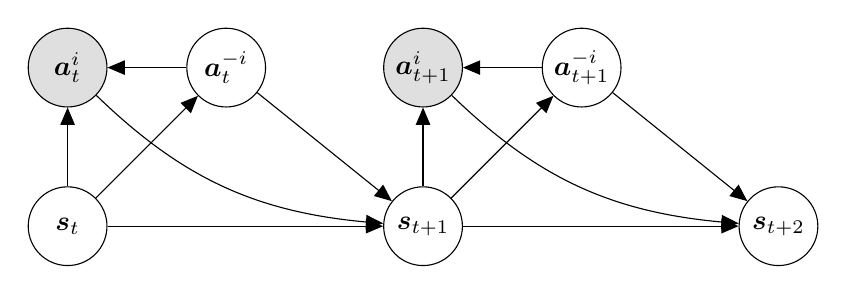
\begin{tikzpicture}[latent/.append style={minimum size=1.0cm}]
        \node[latent] (st) {$\boldsymbol{s}_t$};
        \node[obs, above=of st] (at) {$\boldsymbol{a}^{i}_t$};
        \node[latent, right=of at] (a1t) {$\boldsymbol{a}^{-i}_t$};
        
        \node[latent, right=3.5cm of st] (st1) {$\boldsymbol{s}_{t+1}$};
        \node[obs, above=of st1] (at1) {$\boldsymbol{a}^{i}_{t+1}$};
        
        \node[latent, right=of at1] (a1t1) {$\boldsymbol{a}^{-i}_{t+1}$};
        \node[latent, right=3.5cm of st1] (st2) {$\boldsymbol{s}_{t+2}$};        
        % above right=1.3cm of a
        \edge {st, a1t} {st1}
        \edge {st} {a1t, at}
        \edge {a1t} {at}
        \edge {a1t1} {at1}
        
        \edge{st1} {a1t1, at1}
        \edge {st1, a1t1} {st2}
        
        \path[->]  (at)  edge   [bend right=20] node {} (st1);
        \path[->]  (at1)  edge   [bend right=20] node {} (st2);
    \end{tikzpicture}
    \end{minipage}%
    \begin{minipage}[t]{0.5\linewidth}
    \captionof{figure}{Graphical model that we will fit $\rho_{\phi}$ to get the optimal opponent policy, given that we know the agent's policy.} 
    \end{minipage}
\end{figure}
\noindent
The joint probability is then defined to be 
\begin{equation}
     q'(\boldsymbol{s}_{1:T}, \boldsymbol{a}^i_{1:T}, \boldsymbol{a}^{-i}_{1:T}) = P(\boldsymbol{s}_1) \prod^T_{t=1} P(\boldsymbol{s}_{t+1} | \boldsymbol{s}_{t}, \boldsymbol{a}^i_{t}, \boldsymbol{a}^{-i}_{t}) \pi_{\theta}(\boldsymbol{a}^i_t | \boldsymbol{s}_t, \boldsymbol{a}^{-i}_t) \rho_{\phi}(\boldsymbol{a}^{-i}_t | \boldsymbol{s}_t)
\end{equation}
Similar to agent's case, we now do the variational inference by finding and optimizing ELBO.
\begin{equation}
    \label{equation:18}
    \begin{aligned}
        \log P(\mathcal{O}^{-i}_{1:T} = 1) &= \log \int P(\mathcal{O}^{-i}_{1:T} = 1, \boldsymbol{s}_{1:T}, \boldsymbol{a}^i_{1:T}, \boldsymbol{a}^{-i}_{1:T}) \ d\boldsymbol{s}_{1:T} \ d\boldsymbol{a}^i_{1:T} \ d\boldsymbol{a}^{-i}_{1:T} \\ 
        &= \log \int P(\mathcal{O}^{-i}_{1:T} = 1, \boldsymbol{s}_{1:T}, \boldsymbol{a}^i_{1:T}, \boldsymbol{a}^{-i}_{1:T}) \frac{q'(\boldsymbol{s}_{1:T}, \boldsymbol{a}^i_{1:T}, \boldsymbol{a}^{-i}_{1:T})}{q'(\boldsymbol{s}_{1:T}, \boldsymbol{a}^i_{1:T}, \boldsymbol{a}^{-i}_{1:T})} \ d\boldsymbol{s}_{1:T} \ d\boldsymbol{a}^i_{1:T} \ d\boldsymbol{a}^{-i}_{1:T} \\
        &\ge \mathbb{E}_{q'(\boldsymbol{s}_{1:T}, \boldsymbol{a}^i_{1:T}, \boldsymbol{a}^{-i}_{1:T})}\Bigg[ \log \frac{P(\mathcal{O}^{-i}_{1:T} = 1, \boldsymbol{s}_{1:T}, \boldsymbol{a}^i_{1:T}, \boldsymbol{a}^{-i}_{1:T})}{q'(\boldsymbol{s}_{1:T}, \boldsymbol{a}^i_{1:T}, \boldsymbol{a}^{-i}_{1:T})} \Bigg] \\
        &= \mathbb{E}_{q'(\boldsymbol{s}_{1:T}, \boldsymbol{a}^i_{1:T}, \boldsymbol{a}^{-i}_{1:T})}\Bigg[\sum^{T}_{t=1}  R^{-i}(\boldsymbol{s}_{t}, \boldsymbol{a}^{-i}_{t}) - \log \frac{\rho_{\phi}(\boldsymbol{a}^{-i}_t | \boldsymbol{s}_t)}{P_{\text{prior}}(\boldsymbol{a}^{-i}_t)}\Bigg]
    \end{aligned}
\end{equation}
We refer to section \ref{ELBO:opponent} for more detailed proof of ELBO.
We now repeat the process that find the closed form of opponent's model. Starting of by introducing a normalizing/message term $V^{-i}(\boldsymbol{s}_T)$ at the base case. 
\begin{equation}
    \mathbb{E}_{q'(\boldsymbol{s}_{T}, \boldsymbol{a}^i_{T}, \boldsymbol{a}^{-i}_{T})}\Bigg[\sum^{T}_{t=1}  R^{-i}(\boldsymbol{s}_{t}, \boldsymbol{a}^{-i}_{t}) - \log \frac{\rho_{\phi}(\boldsymbol{a}^{-i}_t | \boldsymbol{s}_t)}{P_{\text{prior}}(\boldsymbol{a}^{-i}_t)} - V^{-i}(\boldsymbol{s}_T) + V^{-i}(\boldsymbol{s}_T)\Bigg]
\end{equation}
With some algebraic manipulation, we got (we can ignore the agent's policy since it doesn't contribute into anything)
\begin{equation}
    \mathbb{E}_{q'(\boldsymbol{s}_{T})} \Bigg[ -D_{KL}\Bigg( \rho_{\phi}(\boldsymbol{a}^{-i}_t | \boldsymbol{s}_t) \Bigg|\Bigg| \frac{\exp\left(R^{-i}(\boldsymbol{s}_{t}, \boldsymbol{a}^{-i}_{t})\right)P_{\text{prior}}(\boldsymbol{a}^{-i}_t)}{\exp V^{-i}(\boldsymbol{s}_T)} \Bigg) + V^{-i}(\boldsymbol{s}_T) \Bigg]
\end{equation}
Now we can comfortably set the opponent's model to be equal to 
\begin{equation}
    \rho_{\phi}(\boldsymbol{a}^{-i}_t | \boldsymbol{s}_t) = \frac{\exp\left(R^{-i}(\boldsymbol{s}_{t}, \boldsymbol{a}^{-i}_{t})\right)P_{\text{prior}}(\boldsymbol{a}^{-i}_t)}{\exp V^{-i}(\boldsymbol{s}_T)}
\end{equation}
With the normalizing term equal to 
\begin{equation}
    V^{-i}(\boldsymbol{s}_T) = \log \int \exp\left(R^{-i}(\boldsymbol{s}_{t}, \boldsymbol{a}^{-i}_{t})\right)P_{\text{prior}}(\boldsymbol{a}^{-i}_t) \ d \boldsymbol{a}^{-i}
\end{equation}
Let's now define opponent model for arbitrary time-step $t$. Given the message passed down from step $t+1$. 
\begin{equation}
    \begin{aligned}
        \mathbb{E}_{q'(\boldsymbol{s}_{t}, \boldsymbol{a}^i_{t}, \boldsymbol{a}^{-i}_{t})} \Bigg[\underbrace{R^{-i}(\boldsymbol{s}_{t}, \boldsymbol{a}^{-i}_{t}) + \gamma\mathbb{E}_{P(\boldsymbol{s}_{t+1}| \boldsymbol{a}^{-i}_{t})}\Big[ V^{-i}(\boldsymbol{s}_{t+1}) \Big]}_{Q^{-i}(\boldsymbol{s}_t, \boldsymbol{a}^{-i}_t)} - \log \frac{\rho_{\phi}(\boldsymbol{a}^{-i}_t | \boldsymbol{s}_t)}{P_{\text{prior}}(\boldsymbol{a}^{-i}_t)} \Bigg]
    \end{aligned}
\end{equation}
Using same method, we also introduce $V^{-i}(\boldsymbol{s}_{t})$ as normalizing terms. Noted that the agent's policy is hidden within the $P(\boldsymbol{s}_{t+1} | \boldsymbol{s}_{t}, \boldsymbol{a}^{-i}_t)$, which is might as well equal to 
\begin{equation}
    P(\boldsymbol{s}_{t+1} | \boldsymbol{s}_{t}, \boldsymbol{a}^{-i}_t) = P(\boldsymbol{s}_{t+1} | \boldsymbol{s}_t, \boldsymbol{a}^i_t, \boldsymbol{a}^{-i}_t) \pi_{\theta}(\boldsymbol{a}^i_t | \boldsymbol{s}_t, \boldsymbol{a}^{-i}_t) \rho_{\theta}(\boldsymbol{a}^{-i}_t | \boldsymbol{s}_t)
\end{equation}
So, now the final opponent model is equal to 
\begin{equation}
    \rho_{\phi}(\boldsymbol{a}^{-i}_t | \boldsymbol{s}_t) = \frac{\exp\left( Q^{-i}(\boldsymbol{s}_t, \boldsymbol{a}^{-i}_t) \right)P_{\text{prior}}(\boldsymbol{a}^{-i}_t)}{\exp V^{-i}(\boldsymbol{s}_{t})}
\end{equation}
Now the rest can be defined as 
\begin{equation}
    \begin{aligned}
        Q^{-i}(\boldsymbol{s}_{t}, \boldsymbol{a}^{-i}_t) &= R^{-i}(\boldsymbol{s}_{t}, \boldsymbol{a}^{-i}_{t}) + \gamma\mathbb{E}_{P(\boldsymbol{s}_{t+1}| \boldsymbol{a}^{-i}_{t})}\Big[ V^{-i}(\boldsymbol{s}_{t+1}) \Big] \\
        V^{-i}(\boldsymbol{s}_{t}) &= \log \int \exp\left( Q^{-i}(\boldsymbol{s}_t, \boldsymbol{a}^{-i}_t) \right)P_{\text{prior}}(\boldsymbol{a}^{-i}_t) \ d\boldsymbol{a}^{-i}_t
    \end{aligned}
\end{equation}

\noindent
\textbf{Claim (1): } $\pi(\boldsymbol{a}^{i} | \boldsymbol{a}^{-i}, \boldsymbol{s})$ isn't \emph{robust}. We defined to term \emph{robust} to be the ability to adapt to difference/unseen opponent model, due to the definition of $Q(\boldsymbol{s}, \boldsymbol{a}^{i}, \boldsymbol{a}^{-i})$, relies on the transition given by opponent models.

\section{Convergence Proof of ROMMEO Balancing Q}




\chapter{Conclusion}
\begin{itemize}
    \item Pure Nash Strategy from VIREL
    \item Graph Neural Network 
    \item Unified View. 
    \item Modeling Belief 
\end{itemize}

\appendix

\bibliographystyle{alpha}
\bibliography{bibilography}

\chapter{Overview of ELBO, EM and Variational Inference}
ELBO or Evidence Lower Bound Objective is one of the most interesting and fruitful objective functions. Its applications span in the from probabilistic generative models \cite{kingma2013auto} to reinforcement learning \cite{levine2018reinforcement}. This section will provides common "pattern" for deriving ELBO, which ultimately leads to Expectation Maximization algorithm, variational inference and variational auto-encoder \cite{kingma2013auto}  \Phu{Cite EM Cite VI add more examples}

Suppose we would like to maximize the probability of generating data point $\boldsymbol{X}$ given the parameter $\boldsymbol{\theta}$. We can assume there exists a latent variable $\boldsymbol{z}$ that generates this data point. Writing it as (assuming $q(\boldsymbol{z})$ is an arbitrary distribution over $\boldsymbol{z}$)

\begin{equation}
    \begin{aligned}
         \log P(\boldsymbol{X} | \boldsymbol{\theta}) &= \int P(\boldsymbol{X}, \boldsymbol{z} | \boldsymbol{\theta}) \ d\boldsymbol{z} \\
         &= \log \int P(\boldsymbol{X}, \boldsymbol{z}) \frac{q(\boldsymbol{z})}{q(\boldsymbol{z})} \ d \boldsymbol{z} \\
         &= \log \mathbb{E}_{\boldsymbol{z} \sim q(\boldsymbol{z})} \left[ \frac{P(\boldsymbol{X}, \boldsymbol{z} | \boldsymbol{\theta})}{q(\boldsymbol{z})} \right] \\
         &\ge \mathbb{E}_{\boldsymbol{z} \sim q(\boldsymbol{z})} \left[ \log\frac{P(\boldsymbol{X}, \boldsymbol{z} | \boldsymbol{\theta})}{q(\boldsymbol{z})} \right]
    \end{aligned}
\end{equation}
The inequality came from Jensen's inequality, hence we arrived at ELBO. The difference between ELBO and $\log P(\boldsymbol{X} |\boldsymbol{\theta})$ is equal to 

\begin{equation}
    \begin{aligned}
        \log P(\boldsymbol{X} |\boldsymbol{\theta}) - &\mathbb{E}_{\boldsymbol{z} \sim p(\boldsymbol{z})} \left[ \log\frac{P(\boldsymbol{X}, \boldsymbol{z} | \boldsymbol{\theta})}{q(\boldsymbol{z})} \right] \\
        &= \log P(\boldsymbol{X} |\boldsymbol{\theta}) - \mathbb{E}_{\boldsymbol{z} \sim q(\boldsymbol{z})}\big[ \log P(\boldsymbol{X}, \boldsymbol{z} | \boldsymbol{\theta}) \big] + \mathbb{E}_{\boldsymbol{z} \sim q(\boldsymbol{z})} \big[ \log q(\boldsymbol{z}) \big]  \\ 
        &= \cancel{\log P(\boldsymbol{X} |\boldsymbol{\theta})} - \mathbb{E}_{\boldsymbol{z} \sim q(\boldsymbol{z})}\big[ \log P( \boldsymbol{z} |\boldsymbol{X} , \boldsymbol{\theta}) \big] - \cancel{\mathbb{E}_{\boldsymbol{z} \sim q(\boldsymbol{z})}\big[ \log P( \boldsymbol{X} | \boldsymbol{\theta}) \big]} + \mathbb{E}_{\boldsymbol{z} \sim q(\boldsymbol{z})} \big[ \log q(\boldsymbol{z}) \big] \\ 
        &=  \mathbb{E}_{\boldsymbol{z} \sim q(\boldsymbol{z})} \big[ \log q(\boldsymbol{z}) \big] - \mathbb{E}_{\boldsymbol{z} \sim q(\boldsymbol{z})} \big[ \log P( \boldsymbol{z} |\boldsymbol{X} , \boldsymbol{\theta}) \big] \\
        &= D_{KL} \left( q(\boldsymbol{z}) || P( \boldsymbol{z} |\boldsymbol{X} , \boldsymbol{\theta}) \right)
    \end{aligned}
\end{equation}
This leads to first optimization step of EM algorithm (E-Step), where the goals of this algorithm is maximizes $\log$ probability. We would like to minimizing the "gap" between ELBO and $P(\boldsymbol{x} | \boldsymbol{\theta})$, therefore in E-Step, we set: 

$$
q(\boldsymbol{z}) \leftarrow P( \boldsymbol{z} |\boldsymbol{X} , \boldsymbol{\theta})
$$

So now, we have that ELBO is equal to $P(\boldsymbol{x} | \boldsymbol{\theta})$, which we now proceeded to maximizing ELBO based on $\theta$, which is equal to optimizing the following objective. 

\begin{equation}
    \arg\max_{\boldsymbol{\theta}} \mathbb{E}_{\boldsymbol{z} \sim q(\boldsymbol{z})}\big[\log P(\boldsymbol{X}, \boldsymbol{z} | \theta)\big]
\end{equation}
We call this step, M-Step. The limitation of EM algorithm lies within in E-Step, suppose, we can't even compute $P( \boldsymbol{z} |\boldsymbol{X} , \boldsymbol{\theta})$ then we have to minimizing the KL distance with respect to parameterized $\phi$ of $q(\boldsymbol{z} | \boldsymbol{X}, \boldsymbol{\phi})$, instead: 

\begin{equation}
    D_{KL}(q(\boldsymbol{z}| \boldsymbol{X}, \boldsymbol{\phi}) || P( \boldsymbol{z} |\boldsymbol{X} , \boldsymbol{\theta}) )
\end{equation}
Which can be shown to be equal to minimizing ELBO for both parameters $\boldsymbol{\phi}, \boldsymbol{\theta}$
\begin{equation}
    \begin{aligned}
        D_{KL}(q(\boldsymbol{z}| \boldsymbol{X}, \boldsymbol{\phi}) || P( \boldsymbol{z} |\boldsymbol{X} , \boldsymbol{\theta}) ) &= \mathbb{E}_{\boldsymbol{z} \sim q(\boldsymbol{z} | \boldsymbol{X}, \boldsymbol{\phi})} \left[ \log \frac{q(\boldsymbol{z} | \boldsymbol{X}, \boldsymbol{\phi})}{P(\boldsymbol{z} | \boldsymbol{X}, \boldsymbol{\theta})} \right] \quad \text{ where } P(\boldsymbol{z} | \boldsymbol{X}, \boldsymbol{\theta}) = \frac{P(\boldsymbol{X} | \boldsymbol{z}, \boldsymbol{\theta}) P(\boldsymbol{z})}{P(\boldsymbol{X} | \boldsymbol{\theta})} \\ 
        &= \mathbb{E}_{\boldsymbol{z} \sim q(\boldsymbol{z} | \boldsymbol{X}, \boldsymbol{\phi})} \left[ \log \frac{q(\boldsymbol{z} | \boldsymbol{X}, \boldsymbol{\phi}) P(\boldsymbol{X} | \boldsymbol{\theta})}{P(\boldsymbol{X} | \boldsymbol{z}, \boldsymbol{\theta}) P(\boldsymbol{z})} \right] \\ 
        &= \underbrace{\mathbb{E}_{\boldsymbol{z} \sim q(\boldsymbol{z} | \boldsymbol{X}, \boldsymbol{\phi})} \left[ \log \frac{q(\boldsymbol{z} | \boldsymbol{X}, \boldsymbol{\phi})}{P(\boldsymbol{X} | \boldsymbol{z}, \boldsymbol{\theta}) P(\boldsymbol{z})} \right]}_{\text{ELBO}} + \mathbb{E}_{\boldsymbol{z} \sim q(\boldsymbol{z} | \boldsymbol{X}, \boldsymbol{\phi})} \left[ \log P(\boldsymbol{X} | \boldsymbol{\theta}) \right]  \\ 
        &= -\mathbb{E}_{\boldsymbol{z} \sim q(\boldsymbol{z} | \boldsymbol{X}, \boldsymbol{\phi})} \left[ \log P(\boldsymbol{X} | \boldsymbol{z}, \boldsymbol{\theta}) \right] + \mathbb{E}_{\boldsymbol{z} \sim q(\boldsymbol{z} | \boldsymbol{X}, \boldsymbol{\phi})} \left[ \log \frac{q(\boldsymbol{z} | \boldsymbol{X}, \boldsymbol{\phi})}{P(\boldsymbol{z})} \right] + \text{const} \\ 
        &= -\mathbb{E}_{\boldsymbol{z} \sim q(\boldsymbol{z} | \boldsymbol{X}, \boldsymbol{\phi})} \left[ \log P(\boldsymbol{X} | \boldsymbol{z}, \boldsymbol{\theta}) \right] + D_{KL}(q(\boldsymbol{z} | \boldsymbol{X}, \boldsymbol{\phi}) || P(\boldsymbol{z})) + \text{const}
    \end{aligned}
\end{equation}
Now we can also arrived at the ELBO objective. We can interpreted optimizing ELBO with respect to $\phi, \theta$ as EM algorithm where optimizing with respect to $\phi$ is an E-Step and optimizing with respect to $\theta$ is an M-Step. This is also used as optimizing objective in Variational Auto Encoder \cite{kingma2013auto}, where we denote $q(\boldsymbol{z} | \boldsymbol{X}, \boldsymbol{\phi})$ as an encoder and $P(\boldsymbol{X} | \boldsymbol{z}, \boldsymbol{\theta})$ as a decoder




\chapter{Soft-Q Learning Objective from Probabilistic Interpretation of Reinforcement Learning}
In the survey \cite{levine2018reinforcement}, the authors provided probabilistic interpretation of reinforcement learning, however, they assume the prior over actions to be uniform. Similarly \cite{grau2018soft} briefly provide and derive objective with explicit prior over actions. In this section, we will go in depth on how to derived such an objective.

We start with assuming a hidden variables $\boldsymbol{a}_{1:T}$ and $\boldsymbol{s}_{1:T}$, where the observed variable to be the optimality $\mathcal{O}_{1:T}$. Given by the following graphical models.

\begin{figure}[!h]
  \tikz{
     \node[obs] (o1) {$\mathcal{O}_1$};
     \node[latent, below=of o1] (a1) {$\bold{a}_1$};
     \node[latent, below=of a1] (s1) {$\bold{s}_1$};
     
     \node[obs, right=of o1] (o2) {$\mathcal{O}_2$};
     \node[latent, right=of a1] (a2) {$\bold{a}_2$};
     \node[latent, right=of s1] (s2) {$\bold{s}_2$};
     
     \node[latent, right=of s2] (s3) {$\bold{s}_3$};
     \node[latent, right=of s3] (st) {$\bold{s}_T$};
     \node at ($(s3)!.5!(st)$) {\ldots};
     
     \path[->]  (s1)  edge   [bend left=30] node {} (o1);
     \edge {a1} {o1}  
     
     \path[->]  (s2)  edge   [bend left=30] node {} (o2);
     \edge {s1, a1} {s2}
     \edge {a2} {o2}
     
     \edge {s2, a2} {s3}
    %  \node[latent,above=of o, xshift=-1cm,fill] (y) {$y$}; 
    %  \node[latent,above=of o,xshift=1cm] (z) {$z$};
    %  \edge {y,z} {o}  
 }
\end{figure}

\Phu{Check this out}
Where we defined the optimality $\mathcal{O}_{1:T}$ to be (Assuming $r$ to always be positive)
\begin{equation}
    P(\mathcal{O}_{t} = 1 | \boldsymbol{s}_{t}, \boldsymbol{a}_{t}) = \frac{\exp\left(\beta \cdot r(\boldsymbol{s}_{t}, \boldsymbol{a}_{t})\right)}{\int \exp(\beta \cdot r(\boldsymbol{s}_{t}, \boldsymbol{a}_{t})) \ d\boldsymbol{s}_{t} d\boldsymbol{a}_{t}}
\end{equation}
And we can see that 
\begin{equation}
    P(\mathcal{O}_{1:T} | \boldsymbol{s}_{1:T}, \boldsymbol{a}_{1:T}) \propto \exp \left( \beta \sum^T_{t=1} r(s_t, a_t) \right)
\end{equation}
Since each optimality variables are conditional independent for each time step. 

We would like to find approximated posterior distribution $q$, which we defined it by probabilistic graphical model as
\begin{figure}[!h]
  \tikz{
     \node[latent] (a1) {$\bold{a}_1$};
     \node[latent, below=of a1] (s1) {$\bold{s}_1$};
     
     \node[latent, right=of a1] (a2) {$\bold{a}_2$};
     \node[latent, right=of s1] (s2) {$\bold{s}_2$};
     
     \node[latent, right=of s2] (s3) {$\bold{s}_3$};
     \node[latent, right=of s3] (st) {$\bold{s}_T$};
     \node at ($(s3)!.5!(st)$) {\ldots};
     
     \edge {s1} {a1}  
     \edge {s1, a1} {s2}
     \edge {s2} {a2}
     
     \edge {s2, a2} {s3}
    %  \node[latent,above=of o, xshift=-1cm,fill] (y) {$y$}; 
    %  \node[latent,above=of o,xshift=1cm] (z) {$z$};
    %  \edge {y,z} {o}  
 }
\end{figure}

The joint probability distribution of $q(\boldsymbol{s}_{1:T}, \boldsymbol{a}_{1:T})$ to be 
\begin{equation}
    q(\boldsymbol{s}_{1:T}, \boldsymbol{a}_{1:T}) = P(\boldsymbol{s}_1)\prod^T_{t=1} P(\boldsymbol{s}_{t+1} | \boldsymbol{s}_t, \boldsymbol{a}_t) \pi_{\theta}(\boldsymbol{a}_t | \boldsymbol{s}_t)
\end{equation}
Now we can minimize the KL-Divergence to perform approximate variational inference.
\begin{equation}
        D_{KL} \Big[ q(\boldsymbol{s}_{1:T}, \boldsymbol{a}_{1:T}) \Big\lvert\Big\rvert P(\boldsymbol{s}_{1:T}, \boldsymbol{a}_{1:T} | \mathcal{O}_{1:T} = 1) \Big] = D_{KL} \left[ q(\boldsymbol{s}_{1:T}, \boldsymbol{a}_{1:T}) \Bigg\lvert\Bigg\rvert \frac{P(\mathcal{O}_{1:T} | \boldsymbol{s}_{1:T}, \boldsymbol{a}_{1:T}) P_{\text{prior}} (\boldsymbol{s}_{1:T}, \boldsymbol{a}_{1:T}) }{P(\mathcal{O}_{1:T})} \right]
\end{equation}
The $P_{\text{prior}}$ is defined to be 
\begin{equation}
    P_{\text{prior}}(\boldsymbol{s}_{1:T}, \boldsymbol{a}_{1:T}) = P(\boldsymbol{s}_1)\prod^T_{t=1} P(\boldsymbol{s}_{t+1} | \boldsymbol{s}_t, \boldsymbol{a}_t) \pi_{\text{prior}}(\boldsymbol{a}_t | \boldsymbol{s}_t)
\end{equation}
Which the evaluation of KL-Divergence yields optimizing the following objective
\begin{equation}
    \begin{aligned}
        \mathbb{E}_{(\boldsymbol{s}_{1:T}, \boldsymbol{a}_{1:T}) \sim q(\boldsymbol{s}_{1:T}, \boldsymbol{a}_{1:T})} &\left[ \log q(\boldsymbol{s}_{1:T}, \boldsymbol{a}_{1:T}) \right] -  \mathbb{E}_{(\boldsymbol{s}_{1:T}, \boldsymbol{a}_{1:T}) \sim q(\boldsymbol{s}_{1:T}, \boldsymbol{a}_{1:T})} \left[ \log \frac{P(\mathcal{O}_{1:T} | \boldsymbol{s}_{1:T}, \boldsymbol{a}_{1:T}) P_{\text{prior}} (\boldsymbol{s}_{1:T}, \boldsymbol{a}_{1:T}) }{P(\mathcal{O}_{1:T})} \right] \\ 
        &= \ \begin{aligned}[t]
           &\mathbb{E}_{(\boldsymbol{s}_{1:T}, \boldsymbol{a}_{1:T}) \sim q(\boldsymbol{s}_{1:T}, \boldsymbol{a}_{1:T})} \left[ \log \left[ P(\boldsymbol{s}_1) \prod^T_{t=1} P(\boldsymbol{s}_{t+1} | \boldsymbol{s}_t, \boldsymbol{a}_t) \pi_{\theta}(\boldsymbol{a}_t | \boldsymbol{s}_t) \right] \right] \\
            &- \mathbb{E}_{(\boldsymbol{s}_{1:T}, \boldsymbol{a}_{1:T}) \sim q(\boldsymbol{s}_{1:T}, \boldsymbol{a}_{1:T})} \big[ \log P(\mathcal{O}_{1:T} | \boldsymbol{s}_{1:T}, \boldsymbol{a}_{1:T}) \big] \\ 
            &- \mathbb{E}_{(\boldsymbol{s}_{1:T}, \boldsymbol{a}_{1:T}) \sim q(\boldsymbol{s}_{1:T}, \boldsymbol{a}_{1:T})} \left[ \log \left[ P(\boldsymbol{s}_1) \prod^T_{t=1} P(\boldsymbol{s}_{t+1} | \boldsymbol{s}_t, \boldsymbol{a}_t) \pi_{\text{prior}}(\boldsymbol{a}_t | \boldsymbol{s}_t) \right] \right] 
        \end{aligned} \\
        &= \begin{aligned}[t]
            &\mathbb{E}_{(\boldsymbol{s}_{1:T}, \boldsymbol{a}_{1:T}) \sim q(\boldsymbol{s}_{1:T}, \boldsymbol{a}_{1:T})} \left[ \log P(\boldsymbol{s}_1) + \sum^T_{t=1} \log P(\boldsymbol{s}_{t+1} | \boldsymbol{s}_t, \boldsymbol{a}_t) + \log \pi_{\theta}(\boldsymbol{a}_t | \boldsymbol{s}_t) \right] \\
            &- \mathbb{E}_{(\boldsymbol{s}_{1:T}, \boldsymbol{a}_{1:T}) \sim q(\boldsymbol{s}_{1:T}, \boldsymbol{a}_{1:T})} \left[ \lambda \sum^T_{t=1} r(\boldsymbol{s}_t, \boldsymbol{a}_t) \right] \\
            &- \mathbb{E}_{(\boldsymbol{s}_{1:T}, \boldsymbol{a}_{1:T}) \sim q(\boldsymbol{s}_{1:T}, \boldsymbol{a}_{1:T})} \left[ \log P(\boldsymbol{s}_1) + \sum^T_{t=1} \log P(\boldsymbol{s}_{t+1} | \boldsymbol{s}_t, \boldsymbol{a}_t) + \log \pi_{\text{prior}}(\boldsymbol{a}_t | \boldsymbol{s}_t) \right]
        \end{aligned} \\ 
        &= \begin{aligned}[t]
            &-\mathbb{E}_{(\boldsymbol{s}_{1:T}, \boldsymbol{a}_{1:T}) \sim q(\boldsymbol{s}_{1:T}, \boldsymbol{a}_{1:T})} \left[\lambda \sum^T_{t=1}  r(\boldsymbol{s}_t, \boldsymbol{a}_t) \right] \\
            &+ \mathbb{E}_{(\boldsymbol{s}_{1:T}, \boldsymbol{a}_{1:T}) \sim q(\boldsymbol{s}_{1:T}, \boldsymbol{a}_{1:T})} \left[ \sum^T_{t=1} \log \pi_{\theta}(\boldsymbol{a}_t | \boldsymbol{s}_t) - \log \pi_{\text{prior}}(\boldsymbol{a}_t | \boldsymbol{s}_t) \right]
        \end{aligned}
    \end{aligned}
\end{equation}

The object we have maximizes becomes:
\begin{equation}
    \lambda \mathbb{E}_{(\boldsymbol{s}_{1:T}, \boldsymbol{a}_{1:T}) \sim q(\boldsymbol{s}_{1:T}, \boldsymbol{a}_{1:T})} \left[\sum^T_{t=1}  r(\boldsymbol{s}_t, \boldsymbol{a}_t) \right] - \sum^T_{t=1} D_{KL}\Big[ \pi_{\theta} (\boldsymbol{a}_t | \boldsymbol{s}_t) \Big|\Big| \pi_{\text{prior}} (\boldsymbol{a}_t | \boldsymbol{s}_t) \Big]
\end{equation}
Noted that if the $\pi_{\text{prior}}$ is uniform distribution, then the objective becomes maximum entropy reinforcement learning.



\chapter{ROMMEO\cite{tian2019regularized}}\label{ROMMEOFull}
\begin{figure}[ht]
    \begin{minipage}[t]{0.5\linewidth}
    \centering
    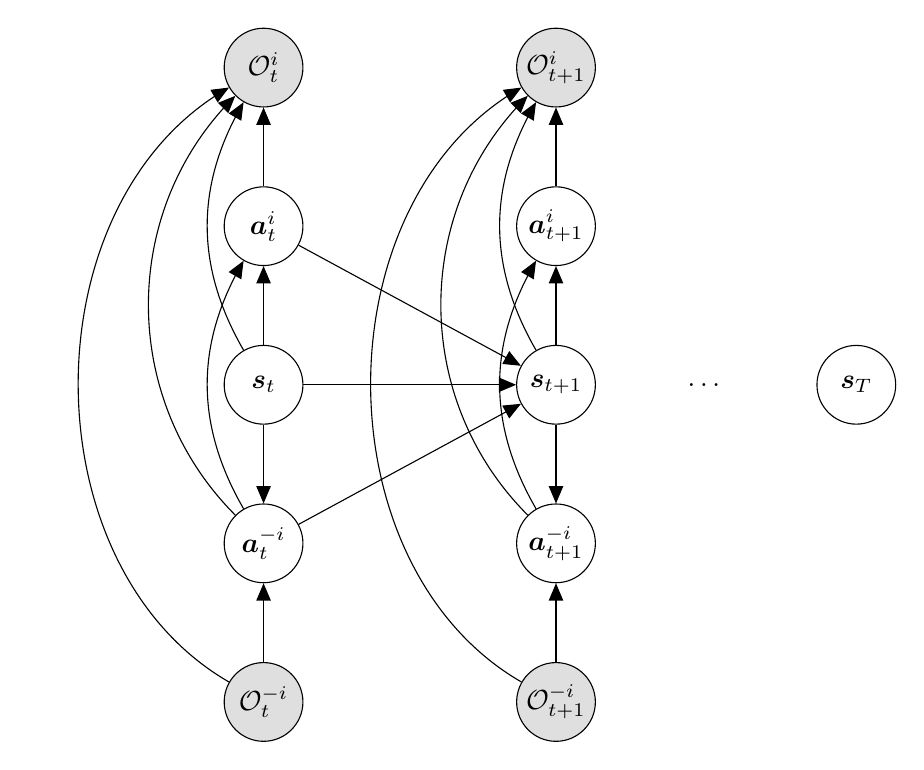
\begin{tikzpicture}[latent/.append style={minimum size=1.0cm}]
        \node[obs] (o) {$\mathcal{O}^i_t$};
        \node[latent, below=of o] (a) {$\boldsymbol{a}^i_t$};
        \node[latent, below=of a] (s) {$\boldsymbol{s}_t$};
        \node[latent, below=of s] (a1) {$\boldsymbol{a}^{-i}_t$};
        \node[obs, below=of a1] (o1) {$\mathcal{O}^{-i}_t$};
        
        \node[obs, right=of o] (o2) [right=2.7cm of o] {$\mathcal{O}^i_{t+1}$};
        \node[latent, right=of s] (s2) [right=2.7cm of s] {$\boldsymbol{s}_{t+1}$};
        \node[latent, right=of a] (a2) [right=2.7cm of a] {$\boldsymbol{a}^i_{t+1}$};
        \node[latent, right=of a1] (a12) [right=2.7cm of a1] {$\boldsymbol{a}^{-i}_{t+1}$};
        \node[obs, right=of o1] (o12) [right=2.7cm of o1] {$\mathcal{O}^{-i}_{t+1}$};
        
        \edge{a, a1, s}{s2}
        
        % \path[->]  (o1)  edge   [bend right=30] node {} (a);
        \edge{o1} {a1}
        \edge {s} {a, a1}
        \edge {a} {o}
        \path[->]  (o1)  edge   [bend left=60] node {} (o);
        \path[->]  (a1)  edge   [bend left=45] node {} (o);
        \path[->]  (a1)  edge   [bend left=30] node {} (a);
        \path[->]  (s)  edge   [bend left=30] node {} (o);
        
        \edge{o12} {a12}
        \edge {s2} {a2, a12}
        \edge {a2} {o2}
        \path[->]  (o12)  edge   [bend left=60] node {} (o2);
        \path[->]  (a12)  edge   [bend left=45] node {} (o2);
        \path[->]  (a12)  edge   [bend left=30] node {} (a2);
        \path[->]  (s2)  edge   [bend left=30] node {} (o2);
        
        \node[latent, right=of s2] (st)[right=2.8cm of s2] {$\boldsymbol{s}_T$};
        
        \node at ($(s2)!.5!(st)$) {\ldots};
        
    \end{tikzpicture}
    \label{ROMMEO-Graphical}
    \end{minipage}%
    \begin{minipage}[t]{0.5\linewidth}
    Graphical model of ROMMEO \cite{tian2019regularized}.Now in the form of stochastic game.
    \end{minipage}
\end{figure}

\end{document}
